% !TEX encoding = UTF-8 Unicode
%
% Niniejszy plik stanowi przykład formatowania pracy magisterskiej na
% Wydziale MIM UW.  Szkielet użytych poleceń można wykorzystywać do
% woli, np. formatujac wlasna prace.
%
% Zawartosc merytoryczna stanowi oryginalnosiagniecie
% naukowosciowe Marcina Wolinskiego.  Wszelkie prawa zastrzeżone.
%
% Copyright (c) 2001 by Marcin Woliński <M.Wolinski@gust.org.pl>
% Poprawki spowodowane zmianami przepisów - Marcin Szczuka, 1.10.2004
% Poprawki spowodowane zmianami przepisow i ujednolicenie
% - Seweryn Karłowicz, 05.05.2006
% Dodanie wielu autorów i tłumaczenia na angielski - Kuba Pochrybniak, 29.11.2016

% dodaj opcję [licencjacka] dla pracy licencjackiej
% dodaj opcję [en] dla wersji angielskiej (mogą być obie: [licencjacka,en])
\documentclass[licencjacka]{pracamgr}
\usepackage{amsmath}
\usepackage{mathtools}
\usepackage{indentfirst}
\usepackage{graphicx}
\usepackage{caption}
\usepackage{float}
\captionsetup{justification=raggedright, singlelinecheck=false}
\usepackage{listings}
\usepackage{amsfonts}
\lstset{
	basicstyle=\small\ttfamily,
	columns=flexible,
	breaklines=true
}
\DeclareMathOperator*{\argmax}{arg\,max}
\newcommand{\norm}[1]{\left\lVert#1\right\rVert}

% Dane magistranta:
\autor{Marcin Basiuk}{mbp-18217}

\title{Przegląd wybranych algorytmów uczenia maszynowego i sztucznej inteligencji na przykładzie gry w kółko i krzyżyk}


%\tytulang{Przegląd wybranych algorytmów uczenia maszynowego
%oraz sztucznej inteligencji na przykładzie gry w kółko i krzyżyk}

%kierunek:
% - matematyka, informacyka, ...
% - Mathematics, Computer Science, ...
\kierunek{Data Science w zastosowaniach biznesowych.
Warsztaty z wykorzystaniem programu R.}

\opiekun{dr. Piotr Wójcik\\
  Zakład Finansów Ilościowych\\
 }

% miesiąc i~rok:
\date{Czerwiec 2018}

%Podać dziedzinę wg klasyfikacji Socrates-Erasmus:
\dziedzina{}

%Klasyfikacja tematyczna wedlug AMS (matematyka) lub ACM (informatyka)
\klasyfikacja{
%D. Software\\
%  D.127. Blabalgorithms\\
%  D.127.6. Numerical blabalysis
}

% Słowa kluczowe:
\keywords{mimimax,teoria gier, uczenie maszynowe, sieci neuronowe, reinformcent learning, procesy markowa }

% Tu jest dobre miejsce na Twoje własne makra i~środowiska:
\newtheorem{defi}{Definicja}[section]

% koniec definicji

\begin{document}

\maketitle
%tu idzie streszczenie na strone poczatkowa
\begin{abstract}
  W pracy zaimplementowano trzy różne algorytmy uczące komputer gry w kółko i krzyżyk. Pierwszym algorytmem jest Minimax połączony z przycinaniem $\alpha$ - $\beta$. Następny algorytm, to znany pod angielską nazwą \textit{Q-learning} w połączeniu z  klaysczną tablicą. Trzecie podejcie wykorzystuje sieć neuronową. Praca zawiera opis, porównanie działania algorytmów oraz opis aplikacji do gry z komputerem wykorzystującym wybrane algorytmy.
\end{abstract}

\tableofcontents

%\listoffigures
%\listoftables

\chapter*{Wprowadzenie}
\addcontentsline{toc}{chapter}{Wprowadzenie}

W trakcie zajęć na studiach podyplomowych wiele uwagi poświęcone było budowaniu modeli predykcyjnych. Pracując z  programem R  i RStudio tworzono modele i szacowano parametry tych modeli, tak żeby ,,na końcu'' mieć narzędzie, albo posługując się programistyczną nomenklaturą funkcję, która przyjmuje dane wejściowe i zwraca predykcję na podstawie tych danych. Wykorzystywano w tym celu szereg metod, zaczynając od regresji liniowej lub regresji logistycznej jeżeli zmienna objaśniana miała charakter nominalny, drzewa decyzyjne,  algorytmy k - najbliższych sąsiadów, analizę głównych składowych, czy w końcu sieci neuronowe.  \\

Doświadczenie z zajęć jednoznacznie wskazywało na dwa kluczowe aspekty, które decydowały o skuteczności modeli predykcyjnych. Po pierwsze jakość danych. Zaszumienie danych, bądź niepoprawne skalowanie prowadziło najczęściej do wyników poniżej oczekiwań. Druga sprawa dotyczyła tego na ile zmienne objaśniające rzeczywiście determinują zmienną (lub zmienne) objaśniane. Intuicyjnie, mało kto uwierzy, że dane ankietowe dotyczące średniej ilości godzin spędzonych w pracy połączonych z danymi demograficznymi takimi jak wiek, poziom wykształcenia, miejsce zamieszkania itd. będzie determinować poziom przychodu. Sukces finansowy najprawdopodobniej zależy również od szeregu cech osobowości takich jak odwaga do podążania za swoimi celami, umiejętność budowania swojej pozycji w systemach społecznych itp.  Modele bazujące na danych ankietowych i demograficznych - takie jak budowano na zajęciach - miały skuteczność mierzoną średnim odchyleniem kwadratowy rzędu $70\% - 85\%$  Trudno jednoznacznie powiedzieć na ile satysfakcjonujące są takie wyniki. Można uznać, że model ,,działa'', można też w ten sposób porównywać modele, ale trudno powiedzieć na ile ,,uchwycono'',  prawa natury rządzące poziomem przychodu.\\
 
Podczas przymiarek do napisania tej pracy celem było skoncentrowanie się bardziej na algorytmach uczących komputery, aniżeli na zbieraniu, czyszczeniu i doborze danych, czyli na tzw. ,,feature engineering'''. Należy podkrelić,  że w żadnym wypadku nie pomniejsza się wagi ani znaczenia tej sztuki. Po prostu sam proces towrzenia lagorytmów uczeąych się wydawał się ciekawszy od zbierania i oróbki odpowiednich danych, żeby to uczenie było skuteczne. W poszukiwaniu problemów, w których dane byłyby niejako naturalnie dostępne uwaga autora skupiła się na grach. Jak nauczyć komputer grać w prostą grę?  W tym wypadku dane są zbierane poprzez grę komputera z człowiekiem, z graczem losowym lub z samym sobą (komputer vs. komputer) i oczywiście nie ma mowy o żadnym zaszumieniu. Szachy i warcaby wydawały się zbyt ambitnym wyzwaniem. W obszarze rozważań znalazły się gry karciane, ale lepiej skupiać się na grze w pełni deterministycznej, w której losowość nie miałaby wpływu na wynik. Dzięki temu wiadomo na ile komputer dobrze nauczył się grać, bez względu na to jak dobra trafiła mu się karta. Ostatecznie wybór padł na kółko i krzyżyk - prosta i w pełni deterministyczna gra. Idealne pole do eksperymentowania z algorytmami uczącymi się. \\

W pierwszym rozdziale opisano zaimplementowany algorytm minimax - jest to klasyczne podejście stosowane do uczenia komputerów grania w gry turowe, gdzie jest dwóch graczy i jeżeli jeden wygrywa, to drugi przegrywa; ewentualnie może być remis.  Można polemizować na ile minimax wpisuje się w uczenie maszynowe. Jednak skoro uczy się takiego podejścia na przedmiocie "Artificial Inteligence"  na MIT \cite{MIT_AI},  to wydaje się, żeby pasuje przedmiotowo do niniejszej pracy.\\

W kolejnych dwóch rozdziałach zaprezentowano algorytmy typowe dla ,,reinforcement learning'' (RL). Kiedy komputer uczy się grać w kółko i krzyżyk, to po wykonaniu ruchu, o ile ruch nie kończy gry,  nie ma natychmiastowej informacji zwrotnej, czy to był dobry ruch, czy też zły ruch. W tym sensie, uczenia komputera gry w kółko i krzyżyk (oraz w inne gry) nie wpisuje się w schemat uczenia z nadzorem. Nie wpisuje się również w uczenie bez nadzoru, bo w przypadku gry, możemy na końcu powiedzieć kto wygrał, a kto przegrał. Z pomocą przychodzi RL, o którym Richard S. Sutton i Andrew Barto w swojej książce \cite{RL} piszą, że jest innym paradygmatem uczenia maszynowego, wychodzącym poza uczenie z nadzorem i bez nadzoru.  W rozdziale drugim komputer ucząc się grać w kółko i krzyżyk będzie szacował prawdopodobieństwo wygrania z danego stanu gry i będzie te wartości zapisywał te dane w pliku tekstowym, do którego również odwołuje się w kolejnych grach. Takie podejście staje się niemożliwe w przypadku gier z bardzo dużą przestrzenią stanów (np. szachy, czy GO). Plik byłby zbyt duży i przeszukiwanie pliku zajmowałoby za dużo czasu. W takim wypadku można zaimplementować sieć neuronową, które będzie szacować prawdopodobieństwa wygrania. To ostatnie podejście opisane zostało w rozdziale trzecim. \\

Ponieważ uwaga skupia się na  algorytmach i ich implementacji, postanowiono wykorzystać uniwersalny obiektowy język programowania. Decyzja padła na Python 2.7, który w odczuciu autora łatwiej umożliwia tworzenie i obsługę klas obiektów od R.  Do pracy dołączono również kody źródłowe napisane w języku Python 2.7.


\chapter{Minimax}\label{r:Minimax}


\section{Opis algorytmu}

W takich grach jak kółko i krzyżyk, szachy lub warcaby można mówić o przestrzeni stanów gry. Każdy stan  gry jest reprezentowany przez położenie pionków albo rozmieszczenie kółek i krzyżyków na kwadratowej planszy z 9 polami. Za każdym ruchem, jednego z dwóch graczy, gra przechodzi do innego stanu. Wszystkie możliwe gry są reprezentowane przez drzewo (drzewo w sensie teorii grafów), którego korzeniem jest początkowy stan gry, a kolejne pokolenia, reprezentują na przemian, możliwe ruchy graczy.  Każda ścieżka od korzenia do wybranego liścia  odpowiada jednej w pełni rozegranej grze. I na odwrót, każda możliwa realizacja gry ma odpowiadającą jej ścieżkę na drzewie gry.  Koncepcja ta  jest zilustrowana na poniższym rysunku \ref{Rys1} zaczerpniętym z książki \cite{RL} \\
\begin{center}
	\begin{figure}[h!]
	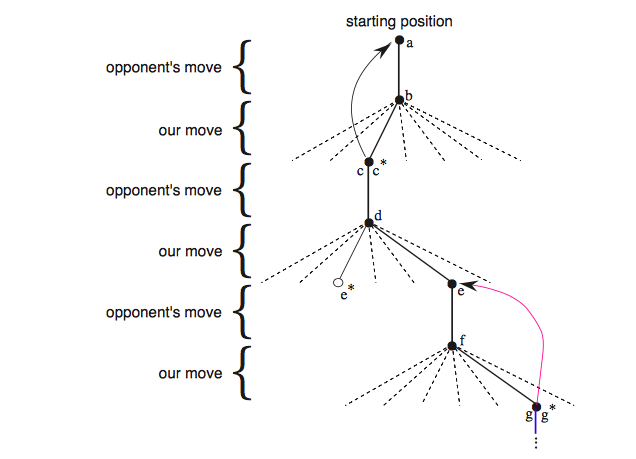
\includegraphics [scale=0.60] {game_tree.png}
	\caption{Drzewo gry}
	\label{Rys1}
	\end{figure}
\end{center}

Przypuśćmy dalej, że z każdym stanem końcowym gry (liściem) można powiązać liczbę wygranych punktów. W przypadku gier takich jak kółko i krzyżyk, może to być jedna z trzech wartości ${-1, 0, 1}$  odpowiadająca przegranej, remisowi i wygranej odpowiednio.  Można jednak wyjść poza ten schemat i rozważać dla stanów końcowych wiele innych wartości.  Ważne jest to, że celem gracza jest maksymalizacja zdobytych punktów. Warto jeszcze zaznaczyć, że punkty przypisane do liści są różne dla rywalizujących ze sobą graczy. W rozpatrywanych  przypadku gry w kółko i krzyżyk, suma punktów zdobytych przez jednego rywala, będzie równa sumie punktów zdobytych przez drugiego rywala, ale z przeciwnym znakiem.  W ogólnym. przypadku jednak tak nie musi być. \\

 Można by naiwnie przypuszczać, że najlepszą strategią będzie wybieranie takiego ruchu, który ,,otworzy'' graczowi ścieżkę do liści z największą możliwą ilością punktów.  Na poniższym przykładzie wziętym ze strony \cite{Game} widać, że taka strategia nie jest optymalna. Wyobraźmy sobie dwie konkurujące ze sobą firmy, które rozważają poniesienie wydatków na promocję oferowanego przez siebie produktu. Firma 1 pierwsza będzie podejmować decyzję, czy inwestować w reklamę, czy też nie.  Ta decyzja odpowiada pierwszemu rozgałęzieniu na poniższym drzewie. Kolejna decyzja  należy do firmy drugiej - inwestować w reklamę lub nie. W sumie są cztery możliwe sytuacje (cztery różne rozgrywki) i odpowiadające im punkty (można je interpretować np. jako zysk). \\

\begin{center}
	\begin{figure}[h!]
	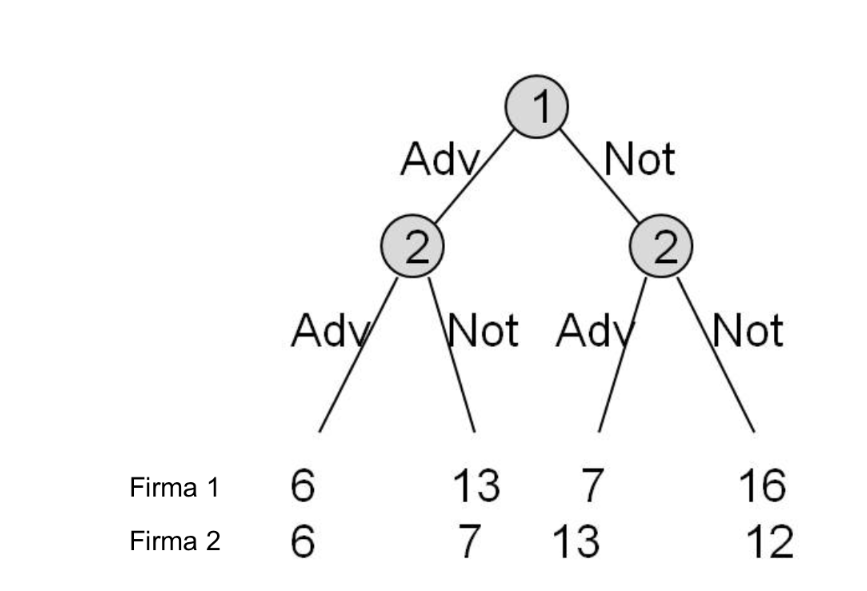
\includegraphics [scale=0.30] {advertise.png}
	\caption{Drzewo decyzyjne dla inwestowania w reklamę}
	\label{Rys2}
	\end{figure}
\end{center}
 
 Jeżeli obie firmy nie zdecydują się nie inwestować w reklamę, to firma 1 zdobędzie 16 punktów, a firma 2 - 12 punktów. Przyjmijmy, że koszt reklamy to 8 punktów. Jeżeli jedna firma zdecyduje się na reklamę, a druga nie, to firma reklamująca uzyska 13 punktów, a firma która nie reklamowała swojego produktu 7 punktów (firma reklamująca się zdobywa 21 punktów z 28 dostępnych, ale ponosi 8 punktowy koszt reklamy).  Natomiast jeżeli obie firmy zdecydują się na reklamę, to podzielą między siebie rynek po równo, ale ponieważ każda z nich poniesie koszt 8 punktów, to finalnie każda zarobi po 6 punktów ($(28 - 16)/2$).\\
 
 Stawiamy się w pozycji prezesem firmy 1, który chce podjąć decyzję o tym, czy inwestować w reklamę czy też nie. Załóżmy dalej, że drzewo przedstawiające możliwe wyniki tej gry jest znane wszystkim zainteresowanym stronom. Wówczas logicznym będzie następujące rozumowanie. Jeżeli firma 1 zdecyduje się na reklamę, to firma 2 chcąc maksymalizować liczbę zdobytych punktów nie będzie się reklamować. Wówczas firma 1 zdobędzie 13, a firma 2  - 7 punktów.  Z drugiej strony, jeżeli firma 1 zdecyduje się nie reklamować, to firma 2 znowu maksymalizując swoją wygraną zainwestuje w reklamę i końcowy wynik będzie 7 i 13 punktów dla firmy 1 i firmy 2 odpowiednio.  Ponieważ pierwszy scenariusz jest korzystniejszy, to firma 1 decyduje się na inwestycję w reklamę. \\
 
 Z powyższego, bardzo prostego rozumowania, wynika kilka wniosków. Po pierwsze, przy założeniu, że oponent (firma 2 w tym przypadku) racjonalnie usiłuję maksymalizować liczbę zdobytych punktów, to wybór ,,otwierający'' drogę do liści z największą liczbą punktów nie musi być wyborem optymalnym. Firma 1 mogłaby zdecydować nie reklamować się, bo wówczas jej potencjalna wygrana, to 7 lub 16 punktów versus 6 i 13 przy reklamowaniu się. Taka strategia byłaby słuszna gdyby firma 2 losowo podejmowała decyzje, ale nie jeżeli firma  2 ma racjonalnych decydentów. Druga obserwacja, często podnoszona w teorii gier, że najlepsze rozwiązanie dla obydwu firm - nie reklamować swoich produktów  - jest rozwiązaniem niemożliwym lub przynajmniej nie stablinym. Teoretycznie prezesi firm mogliby się zmówić, że nie będą inwestować w reklamę.  Ale w takiej sytuacji, o ile firma 1 rzeczywiście zdecyduje nie reklamować się, to firma 2, chcąc maksymalizować swoje punkty, powinna zdecydować się na reklamę i tym samym złamać umowę. Stąd wspomniana wyżej niestabilność.\\
 
Na powyższym przykładzie można też zrozumieć w jaki sposób wybrać optymalny ruch. Załóżmy, że reprezentujmy firmę 1. Do nas należy otwierający ruch. Racjonalnie będzie założyć, że po naszym ruchu firma 2 wykona ruch, który pozwoli w ostatecznym rachunku na maksymalizację jej wygranej, co przy stałej puli możliwych do wygrania punktów, będzie tożsame z takim ruchem, który zminimalizuje naszą wygraną. Zatem należy wybrać taki ruch, który maksymalizuje minimum z naszych wygranych do jakich może doprowadzić firma 2 kolejnym ruchem.  To rozumowanie naturalnie przekłada się na gry, których drzewa mają więcej pokoleń. W każdym przypadku konieczne jest przejście wszystkich węzłów drzewa idąc od liśc (tutaj wiadomo jakie są wygrane) biorąc pod uwagę dla każdego pokolenia czy to ruch gracza (,,nasz ruch''), czy też ruch oponenta, który ma na celu minimalizowanie naszej wygranej. Przedstawiając powyższe rozumowanie w punktach dochodzi się do algorytmu minimax, który dla każdego węzła zwraca wygraną wartość gracza (wygraną pod warunkiem stosowania strategii minimax). \\

\begin{enumerate}
	\item{Jeżeli to jest ruch końcowy, to zwróć wartość wygranej i skończ}
	\item{Jeżeli ruch należy do nas, a nie do oponenta to:}
	\begin{enumerate}
		\item{ustawa wartość$=-\infty$}
		\item{Dla każdego możliwego dostępnego ruchu: }
		\item{wartość = max(wartość,  wartość algorytmu minimax na poddrzewie, którego korzeniem jest rozpatrywany ruch oponenta}
		\item{zwróć wartość}
	\end{enumerate}
		\item{Jeżeli ruch należy do oponenta to:}
	\begin{enumerate}
		\item{ustawa wartość$=+\infty$}
		\item{Dla każdego możliwego dostępnego ruchu: }
		\item{wartość = min(wartość,  wartość algorytmu minimax na poddrzewie, którego korzeniem jest rozpatrywany ruch dla nas}
		\item{zwróć wartość}
	\end{enumerate}
\end{enumerate}


Okazuje się, że jeżeli gracze stosują się do powyższego algorytmu, to znaczy wybierają ruchy, które zapewnią im największą wygraną wyliczoną według powyższego algorytmu, to takie strategie będą w równowadze Nash'a. Mówiąc obrazowo są  to najlepsza strategie, w tym sensie, że żadnemu z graczy nie opłaca się ich zmieniać. Jeżeli wiadomo, że oponent będzie grał zgodnie z algorytmem minimax, to moją najlepszą strategią jest robić to samo. Jeżeli  oponent będzie grał inną strategią, to być może istnieje lepsza odpowiedź na jego strategie niż minimax. Jeżeli gracz gra według algorytmu minimax, a jego oponent nie, to oponent stosuje strategię suboptymalną. 

\section{Przycinanie $\alpha$ - $\beta$}
Podstawowym problemem w zastosowaniach algorytmu minimax jest ilość niezbędnych operacji przy dużych drzewach reprezentujących gry.  Dla gry w kółko i krzyżyk, górnym ograniczeniem ilości możliwych gier (liści na drzewie gry) jest $9! = 362880$. W rzeczywistości ilość możliwych partii ogranicza się do kilku tysięcy, ale i tak przeliczenie wszystkich węzłów takiego drzewa na współczesnym komputerze średniej klasy zajmuje kilka sekund (przynajmniej przy amatorskiej implementacji autora niniejszej pracy). Jeżeli pomyśleć o grach takich jak szachy, w których ilość możliwych ruchów i łączna ilość ruchów w grze jest ogromna, to jasnym się staje, że algorytm minimax ma poważne ograniczenia.  \\

W praktyce, żeby ograniczyć ilość wykonywanych operacji stosuje się tzw. przycinanie  $\alpha$ - $\beta$. Polega to na tym, że jeżeli wiadomo, że sprawdzenie i porównanie wartości dla kolejnego ruch/węzła na drzewie gry nie zmieni wyboru gracza , to pomija się takie obliczenie. Najlepiej zobaczyć to (patrz rysunek \ref{Rys3}) na prostym przykładzie. 

\begin{figure}[h!]
	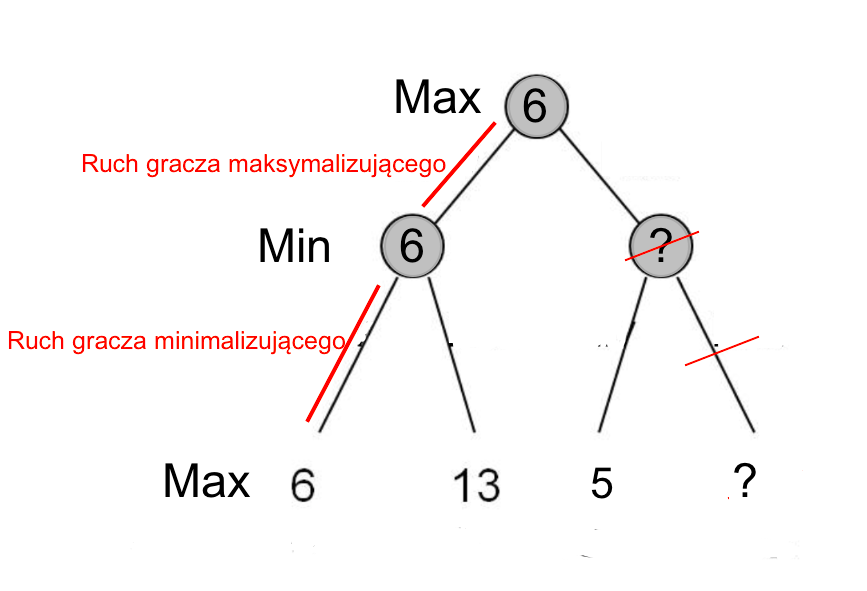
\includegraphics [scale=0.3] {advertise2.png}
	\caption{Przycinanie $\alpha - \beta$}
	\label{Rys3}
\end{figure}

W tym przykładzie gracz rozpocznający grę chce maksymalizować swoją wygraną. W pierwszym ruchu ma dwie możliwości. Może pójść w lewo i wówczas jego oponent z pewnością wybierze lewy skrajny liść i gracz maksymalizujący uzyska wygraną 6. Następie gracz maksymalizujący rozpatruje pierwszy ruch w prawo. Skoro drugi od prawej liść daje wygraną 5, to skrajnego prawego liścia nie ma sesnu już rozważać. Jeżeli tam wygrana byłaby mniejsza od 5, to z punktu widzenia gracza maksymalizującego lepiej wykonać pierwszy ruch w lewo. Ale nawet, gdyby wygrana w prawym skrajnym liściu była bardzo duża (np. 1000), to i tak jest nie osiągalna, bo oponent wybierze liść z wygraną 5. Tak więc w każdym przypadku, pierwszy ruch w lewo, jest dla gracza maksymnalizującego optymalny. Tym samym udało się wyłączyć kawałek drzewa gry z rozważań i zaoszczędzić trochę  operacji przy wykonaywaniu algorytmu minimax. \\

Załóżmy, że mamy do czynienia z takim drzewem gry jak na rysunku \ref{Rys34}. Ostatni wiersz przedstawia możliwe wygrane gracza maksymalizującego, rozpoczynającego grę. Na rysunku zaznaczono węzły i całe podrzewa, których gracz maksymalizujący nie potrzebuje rozpatrywać. Po lewej stronie węzłów zapisana jest maksymalna możliwa wygrana gracza maksymalizującego o ile gra znajdzie się w tym węźle (czyli wartość jaką zwraca algorytm minimax). Pogrubioną linią widać optymalną ścieżkę gry, która kończy się zdobyciem 8 punktów. Opis rozumowania prowadzący do tego rysunku byłby długi i nie wiele wnoszący do całości pracy, stąd zostaje pominięty. Przykład ten wzięty jest z 6 wykładu profesora Winstona z \cite{MIT_AI}.\\

\begin{figure}[h!]
	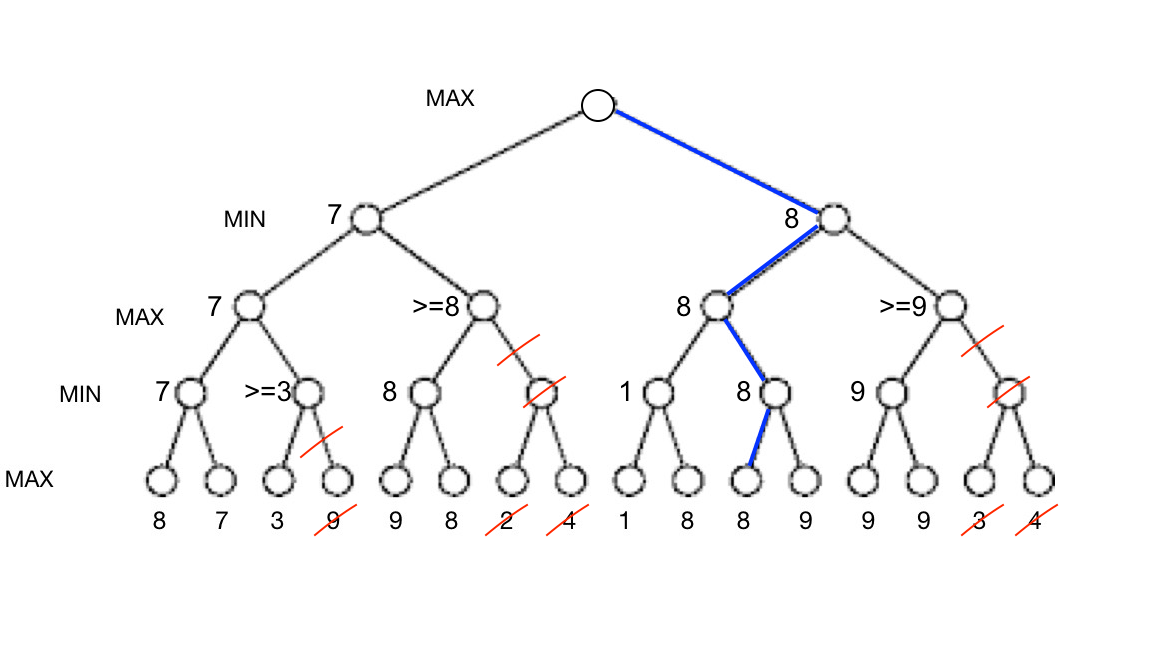
\includegraphics [scale=0.7] {big_tree2.png}
	\caption{Przycinanie $\alpha - \beta$ po raz drugi}
	\label{Rys4}
\end{figure}


Jak widać, w niektórych przypadkach udaje się sporo zaoszczędzić w ilości obliczeń.  Warto jeszcze wyjaśnić skąd $\alpha - \beta$ w nazwie. Zaczynając przeszukiwanie drzewa ustawia się parametry $\alpha$ i $\beta$ na $+\infty$ i $-\infty$ odpowiednio, i interpretuje się je jako najgorszy możliwy wynik gracza minimalizującego ($+\infty$) i  najgorszy możliwy wynik gracza maksymalizującego ($-\infty$). Przechodząc rekurencyjnie przez drzewo sprawdza się aktualizuje wartości $\alpha$ i $\beta$ i jeżeli dla danego poddrzewa  nie możemy poprawić wyniku  $\alpha$ lub  $\beta$ (w zależności czy dla tego poddrzewa pierwszy ruch należy do gracza minimalizującego lub maksymalizującego), to nie przeszukujemy dalej tego poddrzewa.


\section{Funkcja wartości}
Nietrudno wyobrazić sobie, że dla gier z olbrzymimi drzewami gry, przycinanie $\alpha$ - $\beta$ pomoże nam zejść o o kilka pokoleń w dół drzewa, ale i tak nawet najszybszy komputer nie jest w stanie przeszukać całego drzewa w takiej grze jak szachy. W związku z tym,  algorytmy grające w takie gry wykorzystują \textbf{funkcję wartości}. Jest to funkcja zwracająca pewną wartość (scoring) dla każdego stanu gry. Czym wyższa wartość, tym bardziej korzystna sytuacja dla gracza. \\

Algorytm grający będzie z reguły miał ustawiony parametr, który każe przerwać przeszukiwanie drzewa na danym poziomie lub po przekroczeniu określonej ilości czasu. Następnie dla wszystkich liści z przeszukanego poddrzewa do momentu zastopowania algorytmu oblicza się funkcję wartości i w ten sposób estymuje się optymalny ruch.  Dla szachów funkcja wartości może np. zliczać ilość punktów (każda figura ma przypisaną liczbę punktów - pionek 1, koń 5 , wieża 8 itd)  gracza i oponenta figur będących na planszy. 


\section{Implementacja}
 W tej sekcji opisanych zostało  kilka spostrzeżeń związanych z implementacją algorytmu minimax z przycinaniem $\alpha - \beta$.\\

Zastosowanie przycinania $\alpha - \beta$, wbrew pokładnych nadziejom, nie zmniejszyło drastycznie  czasu wykonania algorytmu. Najdłuższy czas oczekiwania ma miejsce na początku gry, w pierwszych dwóch ruchach,  kiedy konieczne jest przeszukanie największych drzew. Od trzeciego ruchu, wykonanie algorytmu trwa poniżej $0.1$ sekundy, więc optymalizacje przestają mieć znaczenie.  Żeby ograniczyć czas oczekiwania na odpowiedź komputera dodałem instrukcję, powodującą, że jeżeli algorytm zaczyna grę, to zawsze wybiera środkowe pole.\\

Nie udało się też zaimplementować algorytmu z ograniczeniem głębokości przeszukiwania drzewa i wykorzystującego funkcję wartości. Banalne funkcje wartości typu sprawdzenie,  czy mam dwa krzyżyki(kółka) w linii nie dawały dobrych rezultatów. Tak skalibrowany algorytm popełniał oczywiste błędy i łatwo z nim było wygrać.  Natomiast uwzględnienie większej ilości niuansów, w zasadzie prowadziło do napisania reguły jak grać w kółko i krzyżyk. Wówczas minimax przestaje być potrzebny i można się ograniczyć do do policzenia funkcji wartości dla możliwych ruchów i wybrania tego z największą wartością. Niestety nie udałosię znaleźć ,,złotego środka'' i w końcowa implementacja nie korzysta z funkcji wartości. \\

Algorytm minimax jest graczem optymalnym, nie można grać lepiej od algorytmu minimax. W szczególności, można co najwyżej z nim zremisować. W dalszej części pracy algorytm minimax będzie obok gracza losowego (takiego co losuje z jednostajnym prawdopodobieństwem kolejny ruch z puli możliwych) punktem odniesienie skuteczności algorytmu grającego w kółko i krzyżyk. Skuteczne algorytmy powinny często remisować i rzadko przegrywać z minimax, oraz często wygrywać i rzadko remistować z graczem losowym. Poniżej przedstawiano wyniki partii 100 gier rozegranych pomiędzy graczem stosującym minimax oraz graczem losowym  oraz 100 gier rozegranych pomiędzy dwoma graczami stosującymi algorytm minimax.\\ 

\begin{figure}[h!]
	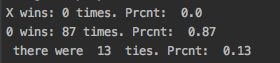
\includegraphics [scale=0.6] {random_minimax.png}
	\caption{Gracz losowy vs minimax}
	\label{Rys5}
\end{figure}

Gracz stosujący minimax nie przegrał ani razu, za to zremisował z graczem losowym 13 razy na 100 gier co ilustruje rysunek \ref{Rys5}. 
Natomiast dwóch graczy stosujących minimax zawsze będą ze sobą remisować (rysunek \ref{Rys6}). 

\begin{figure}[h!]
	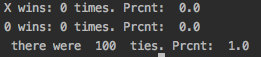
\includegraphics [scale=0.6] {minimax_minimax.png}
	\caption{Gracz minimax vs minimax}
	\label{Rys6}
\end{figure}


\chapter{Q-learning}\label{r:Tablica}

\section{Procesy decyzyjne Markowa}
W rozdziale pierwszym gry były reprezentowane (a w zasadzie wszystkie możliwe rozgrywki) za pomocą drzew, gdzie węzły należały do możliwych stanów gry, a krawędź pomiędzy dwoma węzłami oznaczała przejście na skutek ruchu jednego z graczy do kolejnego stanu. W tym rozdziale zaprezentowany zostanie inny modelu, oparty na procesach decyzyjnych Markowa.  Przed formalnymi definicjami pomocny może okazać się poglądowy rysunkiem wziętym z \cite{RL} oraz  heurystyczny opis modelu.\\

\begin{figure}[h!]
	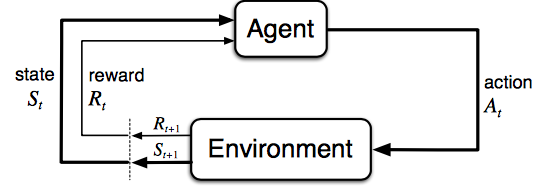
\includegraphics [scale=0.6] {agent_env.png}
	\caption{Wzajemne oddziaływanie środowiska i agent w RL}
	\label{Rys7}
\end{figure}

Załóżmy, że mamy agenta (gracza), który jest w interakcji z pewnym systemem (z angielskiego \textit{environment} na rysunku \ref{Rys7}). Agent znajduje się w pewnym stanie $s$, w dyskretnym czasie $t$ i ma do wyboru podjęcie jednej z dostępnych akcji $a\in\mathcal{A}$. Na skutek podjęcia akcji $a$ system odpowiada przejściem do nowego stanu $s'$ oraz nagrodą $r$ (z ang. \textit{reward}) w czasie $t+1$.  Nie jest przy tym powiedziane, że dla konkretnej pary $(s,a)$ system zawsze przejdzie do tego samego stanu $s'$. System może wybierać swoją odpowiedź losowo (czy ogólnie wedle pewnej niedeterministycznej reguły). Podobnie przy przejściu ze stanu $s$ do $s'$ system może zwracać różne nagrody $r$.  Natomiast ważne, jest że przejcie do kolejnego stany $s'$ oraz powiązana z prześjciem nagroda $r$ zależą tylko i wyłącznie od pary $(s,a)$ i nie mogą w  żaden sposób zależeć od poprzednich stanów w jakich system się znajdował. Na tym polega istota ,,markowość", że historia (poza ostatnim ruchem) nie ma znaczenia. W tym miejscu dodaje się jeszcze jedno założenie dotyczące skończonoci  zbioru możliwych stanów systemu. To założenie nie jest konieczne w ogólnej teorii, ale pozwala na daleko idące uproszczenia wykorzystywane w niniejszej pracy.\\

 Interakcja agenta z systemem przez kilka kolejnych kroków począwszy od $t=0$ można przedstawić za pomocą takiej trajektorii:
$$s_{o}, a_{0}, r_{1}, s_{1}, a_{1}, r_{2}, s_{2}, a_{2}, r_{3}, s_{3},...$$

Formalizując pojęcie procedu decyzyjnego Markowa  rozważmy czwórkę postaci $<\mathcal{S},\mathcal{A},\mathcal{R},p>$ gdzie:
\begin{enumerate}
 	\item{$\mathcal{S}$ jest skończonym zbiorem możliwych stanów systemu}
	\item{$\mathcal{A}$ jest zbiorem możliwych akcji. Formalnie $\mathcal{A}$ jest kolekcją zbiorów $\mathcal{A}_{s}$ indeksowaną stanami $s\in\mathcal{S}$. Chodzi o to, że dla różnych stanów systemy dostępne są różne akcje.  Dla uproszczenie pomija się jednak pomijali ten niuans notacyjny i w dalszej części mowa będzie o możliwych akcjach $\mathcal{A}$  pamiętając, że ten zbiór może być ograniczony w zależnoci od konkretnego stanem.}
	\item{$\mathcal{R}\subseteq\mathbf{R}$ jest zbiorem wartości nagród, jakie agent może otrzymać}
	\item{$p:\mathcal{S}\times\mathcal{A}\times\mathcal{R}\times\mathcal{S}\rightarrow [0,1]$ jest funkcją determinującą dynamikę procesu decyzyjnego Markowa. Dla każdej pary stanu i wyboru akcji w czasie $t$ funkcja $p$ określa rozkład prawdopodobieństwa na $\mathcal{R}\times\mathcal{S}$ w czasie $t+1$:  $$p(s, a, s', r) = \mathbf{P}(S_{t+1}=s', R_{t+1}=r | S_{t}=s, A_{t}=a )$$}
\end{enumerate}

Opisany model z powodzeniem można stosować do opisu gry w kółko i krzyżyk (jak również innych turowych gier). Przestrzeń stanów $\mathcal{S}$ w tym wypadku to będą wszystkie możliwe stany gry. Akcje $\mathcal{A}$ to będą wszystkie możliwe ruchy do wykonania przy danym stanie gry. Agentem jest gracz - algorytm, którego usiłuje się nauczyć grać w kółko i krzyży. Systemem natomiast jest drugi gracz - może to być gracz losowy lub gracz stosujący algorytm minimax. Pozostaje jeszcze określenie nagród $\mathcal{R}$. Wybór jest poniekąd arbitralny, ale ponieważ celem będzie maksymalizowanie wartości oczekiwanej nagród, to należy pamiętać, że algorytm wyuczy się osiągania średnio wysokich nagród, a nie wygrywania. \\

Przed przejściem do opisu algorytmu potrzebne będzie jeszcze kilka pojęć. \textbf{Strategią} nazwiemy dowolne mapowanie 
$$\pi : \mathcal{S}\rightarrow\mathbf{P}_{\mathcal{A}} \text{, gdzie } \forall_{s\in\mathcal{S}} \text{ } \pi(s) \text {  jest rozkładem prawdopodobieństwa na } \mathcal{A}$$ 
Innym słowy, strategia $\pi(s)$ mówi o tym jak gracz ma losować (wybierać) akcję $a$ o ile znajduje się w stanie $s$.\\

Celem gracza będzie dążenie do takiej strategii, która maksymalizuje wartość nagród otrzymanych podczas gry.  W procesach decyzyjnych Markowa często stosuje się dyskontowanie przyszłych nagród wybranym czynnikiem $\gamma\leq1$ Wynika to z dwóch powodów. Po pierwsze w zastosowaniach często przyszłe nagrody mają rzeczywiście niższą wartość niż obecnie (jak strumień pieniądza w czasie w matematyce finansowej) a po drugie, interakcja agenta z system może nie być ograniczona ilością ruchów, a wtedy suma przyszłych nagród niezależnie od wyboru strategii $\pi$ może być nieskończona, co uniemożliwia wybranie optymalnej strategii. Jeżeli natomiast maksymalna nagroda jest ograniczona, powiedźmy liczbą $M$, oraz $\gamma<1$, to suma nagród jest z góry ograniczona przez
$$M+\gamma M +\gamma^{2}M+\gamma^{3}M+...  = \frac{M}{1-\gamma}$$
Dla uproszczenia zapisu wprowadza się oznaczenie na sumę przyszłych zdyskontowanych nagród:
$$G_{t} \stackrel{\text{def}}{=} R_{t+1} + \gamma R_{t+2} + \gamma^{2}R_{t+3} +...$$

Wartością stanu $s$ przy strategii $\pi$ jest z definicji 
$$v_{\pi}(s)\stackrel{\text{def}}{=} \mathbb{E}_{\pi}(G_{t}| S_{t} = s) $$

Jest to wartość oczekiwana sumy zdyskontowanych przyszłych nagród pod warunkiem, że stosujemy strategię $\pi$ począwszy od czasu $t$. w którym to czasie system znajdował się w stanie $s$. 

Podobnie zdefiniuje się jeszcze funkcję określającą wartość akcji $a$ podjętą w stanie $s$ jako zdyskontowaną wartość przyszłych nagród przy założeniu, że stosujemy strategię $\pi$, w stanie $s$ i przy wyborze akcji $a$(strategia $\pi$ zadaje rozkład prawdopodobieństwa na $\mathcal{A}$, i w tej definicji zakładamy, że akurat wylosowano konkretną akcję $a$):
$$q_{\pi}(a,s) \stackrel{\text{def}}{=} \mathbb{E}_{\pi}(G_{t}| S_{t} = s, a_{t} = a) $$

Co zatem oznacza znalezienie optymalnej strategii? Intuicyjnie jest to oczywiste. Chcemy mieć strategię, która będzie maksymalizować wartość oczekiwaną sumy przyszłych zdyskontowanych nagród. Formalnie $\pi_{1}\prec\pi_{2}$ jeżeli dla każdego $s\in\mathcal{S}$ zachodzi $$v_{\pi_{1}}(s)\leq v_{\pi_{1}}(s)$$
Powiemy, że $\pi_{*}$ jest optymalna, jeżeli dla każdej strategii $\pi$ zachodzi   $\pi\prec\pi_{*}$ Nietrudno przy tym zauważyć, że jeżeli $\pi_{*}$ jest optymalną strategią, to spełnione będą równiania:


$$\forall s\in \mathcal{S}: v_{\pi_{*}}(s) =\max_{\pi} v_{\pi}(s)$$ $$\forall s\in\mathcal{S}\wedge \forall a\in\mathcal{A}: q_{\pi_{*}}(a,s) = \max_{\pi} q_{\pi}(a,s)$$
Gdyby na przykład  $v_{\pi_{*}}(s)<v_{\tilde{\pi}}(s)$ dla pewnego stanu $s$ i  pewnej $\tilde{\pi}$, to  strategię $\pi_{*}$ można by poprawić grając strategią $\tilde{\pi}$ po napotkaniu stanu $s$ co jest sprzeczne z tym, że   $\tilde{\pi}\prec\pi_{*}$. Poddobnie ma sie rzecz z równaniem $q_{\pi_{*}}(a,s) = \max_{\pi} q_{\pi}(a,s)$.  Znajość $q_{\pi_{*}}(a,s)$ jest z praktycznego punktu widzenia najbardziej porządana, bo daje odpowiedź na kluczowe pytanie - jaką akcję należy wybrać będąc w stanie $s$:\\
$$\argmax_{a}q_{\pi_{*}}(a,s)$$
Dla uproszczenia zapisu, polożmy:
$$v_{\pi_{*}}:=v_{*}\text{ oraz } q_{\pi_{*}}:=q_{*}$$

Dopiero teraz przechodzimy do pytania jak znaleźć optymalną strategię? Jeżeli zbiory  $\mathcal{S}, \mathcal{A}, \mathcal{R}$ są skończone, to znajomość funkcji $p$ daje ,,pełną wiedzę'' o systemie. W szczególności można dokładnie wyliczyć optymalną strategię, bazując na tzw. równiach Bellman'a, które wiążą $v_{\pi}(s)$ z kolejnym stanem systemu $v_{\pi}(s')$

\begin{equation}
	v_{\pi}(s) = \sum_{a}\pi(a|s)\sum_{s',r}p(s,a,s',r)[r +\gamma v_{\pi}(s')] 
\end{equation}
A w przypakdu strategii optymalnej $\pi_{*}$ równanie Bellmana dla $v_{*}(s)$ oraz dla funkcji $q_{*}$ zadane są przez:

\begin{equation}\label{vstar}
	v_{*}(s) = \max_{a}\sum_{s',r}p(s,a,s',r)[r +\gamma v_{*}(s')]
\end{equation}
\begin{equation}\label{qstar}
	q_{*}(a, s) = \sum_{s',r}p(s,a,s',r)[r +\gamma q_{*}(a,s')]
\end{equation}
Wyprowadzenie powyższych wzorów sprowadza się do zastosowaniu kilki przekształceń i manipulowaniua definicją $v_{\pi}$. Nie jest to skomplikowane, ale zostaje pominięte ze względu na zwięzłość pracy. 

Jeżeli wybierze się aritralną  $\pi$, to bazując na równaniu Bellman'a można policzyć $v_{\pi}(s)$ dla wszytskich stanów $s$. Sprowadza się to do rozsupłanie powyższej ,,rekurencji''  prez rozwiązanie 
$|\mathcal{S}|$  (tutaj $|\cdot|$ oznacza liczebność zbioru ) równań liniowych. Takie podejście może się sprawdzić o ile liczba stanów jest niwielka i łatwo jest policzyć bezpośrednio $v_{*}(s)$ lub $q_{*}(a,s)$ korzystając \ref{vstar} i \ref{qstar}.  Jeżeli jednak przestrzeń stanów jest ,,duża'', to  wówczas stosuje się metody iteracyjne do policzneia $v_{\pi}$, bazujące na cyklicznym poprawianiu wartoci $v_{\pi}(s)$ z wykorzystanien równań Bellman'a. Zaczynamy od arbitralnej strategii $\pi$ i arbitralnej funkcji $v_{0}(s)$. Następnie poprawiamy wiele razy wedłu przepisu:

\begin{equation}\label{GPI}
	v_{k+1}(s) = \sum_{a}\pi(a|s)\sum_{s',r}p(s,a,s',r[r+\gamma v_{k}(s)]
\end{equation}

Okazuje się, że takie iteracyjne poprawianie $v_{k}(s)$ zgodnie z \ref{GPI} gwarantuje zbieżnosć punktową $v_{k}(s)\rightarrow v_{\pi}(s)$, przy $k\rightarrow\infty$.\\

Mając (dla pewnej arbitralnej strategii $\pi$) wyestymowaną funkcję $v_{\pi}(s)$  można policzyć  funckję $q_{\pi}(a,s)$ bezposrednio z definicji:
$$q_{\pi}(a,s)=\mathbb{E}_{\pi}(G_{t}| S_{t} = s, a_{t} = a)  =  \sum_{s',r}p(s',r|s, a)[r+\gamma v_{\pi}(s)]$$

Majć powyższe można  ,,poprawiać'' strategię $\pi$ czyniąc z niej $\pi'$ : 

\begin{equation}\label{update1}
	\pi'(s)\stackrel{\text{def}}{=}\argmax_{a}q_{\pi}(a,s)
\end{equation}


Gdyby ograniczyć się tylko do strategii nielosowych, to dla par  $s$ i $a$ o ile będzie $q_{\pi}(s,a)\geq v_{\pi}(s)$, to znaczy, że akcja $a$  dla stanu $s$ jest lepsza aniżeli $\pi(s)$ i można poprawiać strategię: 
$$\pi'(s) =
	\begin{cases}
		a\text{ ,  }s=a,\\			
		\pi(s)\text{ , } s\neq a\\
	\end{cases}
$$

Okazuje się, że takie sukcesywne, naprzemienne wyliczanie $v_{\pi}$, poprawianie na tej podstawie strategii na $\pi'$, następnie znowu estymowanie $v_{\pi'}$ i tak dalej:

\begin{equation}\label{update2}
 	\pi\rightarrow v_{\pi}\rightarrow \pi' \rightarrow v_{\pi'} \rightarrow \pi'' \rightarrow v_{\pi''} \rightarrow...
\end{equation}


prowadzi do optymalnej strategii $\pi_{*}$.  Algorytm ten często nazywany jest GPI od angielskiego \textit{general policy iteration}. Natomiast całe podejście w \cite{RL} nazywane jest programowaniem dynamicznym (z ang. \textit{dynamic programming}). Jest to skuteczne podejście jeżeli dostępna jest  pełna wiedzę o funkcji $p$ oraz jeżeli liczba możliwych stanów nie jest bardzo duża. Najczęściej to podejście sprawdza się przy modelowaniu rzeczywistychy systemów za pomocą procesu decyzyjnego Markowa.\\

Inną interesującą sytuacją jest brak znajomości funkcji $p$ i wówczas celem jest stworzenie algorytmu, który znajduje optymalną strategię doświadczalnie, ucząc się systemu, bez uprzednich założeń odnośnie zasad rządzącyh  jego dynamiką.  Podobnie jak  w sytuacji znajomoci $p$,  zaczyna się od losowej strategii i z każdym cyklem interakcji z systemem (albo po ustalonej liczbie  $n$ cyklach) dostosowuje się strategię na podstawie dotychczasowych obserwacji zgodnie z \ref{update1} i \ref{update2}. To co się zmienia, to kwestia estymacji funkcji $v_{\pi}(s)$ (lub powiązanej z nią $q_{\pi}(a,s)$). Ponieważ $v_{\pi}(s)$ jest definiowana jako wartość oczekiwana, to naturalnym odruchem może być wyliczanie przyszłych nagród po pierwzej wizycie w stanie $s$ podążając za strategią $\pi$ w wielu epizodach iterakcji agenta z system, a następnie uśrednienia otrzymanych wartości nagród. Takie podejście, typowo w stylu monte-carlo, ma poważną wadę w przypadku systemów z dużą ilością stanów, bo potrzeba czasami nierealistycznie dużej próbki danych (epizodów), żeby sensownie policzyć  $v_{\pi}(s)$. A nawet jeżeli ilość epizodów nie jest problem, to konieczne są pewne dodatkowe założenia takie jak konieczność startowania epizodu ze wszystkich możliwych stanów. W przeciwnym razie pewne stany mogą nigdy nie być odwiedzane i nie trudno wówczas mówić o estymacji $v_{\pi}$.  \\
 
 Metodą, poniekąd łączącą, programowanie dynamiczne z metodami w stylu monte carlo, nie wymagającą znajomości funkcji $p$, są metody Q-learning (albo ogólnej z ang. \textit{temporal difference}).  Idea tych metod sprowadza się do tego, że można w każdy kroku, po każdej interakcji agenta z systemem, poprawiać stosowaną przez niego strategię $\pi$ zgodnie ze wzorem
\begin{equation}\label{qlearning1}
   v_{\pi}(s_{t}) := v_{\pi}(s_{t}) +\alpha [R_{t+1} + \gamma v_{\pi}(s_{t+1}) - v_{\pi}(s_{t})]
 \end{equation}
 albo dla funkcji $q$:
\begin{equation}\label{qlearning2}
   q_{\pi}(s_{t}, a_{t}) := q_{\pi}(s_{t},a_{t}) +\alpha [R_{t+1} + \gamma q_{\pi}(s_{t+1}, a_{t+1}) - q_{\pi}(s_{t},a_{t})]
 \end{equation}
 
 W tym wypadku nie potrzeba czekać do końca epizodu (np. do końca gry), żeby zaktualizować $v_{\pi}(s_{t})$ jak w metodach monte carlo. Estymacja $v_{\pi}$  bazuje tylko na otrzymanej nagrodzie i estymacji $v_{\pi}(s_{t+1})$ dla kolejnego stanu. Ponieważ estymacja częściowo bazuje na estymacju, to mżna powiedzieć, że jest to metoda ,,bootstrapowa'''. Jednak tak jak poprzednio, po wyestymowaniu $v_{pi}$ konieczne jest dalsze podążanie algorytmem GPI, czyli suckesywną poprawą strategii $\pi$ zgodnie z \ref{update2} .   W \ref{qlearning1} i \ref{qlearning2}  $\alpha$ jest hiperparametrem algorytmu, często nazywany z angielskiego \textit{learning rate}, a $\gamma$ jest, już wcześniej wsppomnianym, czynnikiem dyskontującym wartość przyszłych nagród. W kolejnym rozdziale opisana jest zastosowanie tego rodzaju algorytmu. \\
 
 Finalnie algorytmem wykorzystanym w tej pracy do nauki gry w kółko i krzyżyk, jest algorytm znany jako Q-learning, opracowany w 1989 przez C. Watkins'a \cite{Watkins} w ramach jego  pacy dokorskiej. Algorytm Q-learning jest o tyle rewolucyjny, że odchodzi od naprzemiennego estymowania $v_{\pi}$ i poprawiania odpowiednio $\pi\rightarrow \pi'$ jako to ma miejsce w klasycznym GPI. W tym przypadku estymuje się bezpośrednio $q_{*}$ zgodnie ze wzorem:
 \begin{equation}\label{qlearning}
 	 q_{*}(s_{t}, a_{t}) := q_{*}(s_{t},a_{t}) +\alpha [R_{t+1} + \gamma \max_{a_{t+1}} q_{*}(s_{t+1}, a_{t+1}) - q_{*}(s_{t},a_{t})]
 \end{equation} 
 
 
%%%%%%%%%%%%%%%%%%%%%%%%%%%%%%%%%%%%%%%%%%%%%%%%%%%%%%%%%%%%%%%%%%%%%%%%%%%%%%%%%%%%%%% 

\section{Opis algorytmu}

Koncepcja algorytmu uczącego się gry w kółko i krzyżyk bazuje na rozgrywaniu wielu gier z graczem losowym stosując nieustannie \ref{qlearning} i tym samym poprawiając szacowanie funkcji $q_{*}$, która definiuje nam optymalną strategię zgodnie ze wzorem

$$\pi(s) = \argmax_{a}q_{*}(s,a).$$

Do tego dochodzi kilka drobnych subtelnosci, takich jak pilnowanie tego, żeby dla stanów końcowych (koniec gry)  kłasć $q_{*}(s,a)=0$ oraz wybieranie losowych ruchów z małym prawdopodobieństwem $\epsilon>0$. Poniżej znajduje się opis algorytmu w punktach:

\begin{enumerate}
	\item{Zaincjalizuje $q(s,a):=0$ dla wszytskich możliwych stanów}
	\item{Rozegraj $N$ gier w kółko i krzyżyk:}
		\begin{enumerate}
			\item{Jeżeli jest ruch agenta w stanie $s$, to wybierz z prawdopodobieństwem $\epsilon$ ruch $a$ maksymalizujący $q(a,s)$ albo wybierz dowolny legalny ruch z prawdopodobieństwem $\epsilon$}
			\item{Jeżeli ruch agenta był ruchem kończącym grę, to połóż $q(s,a)=0$}
			\item{Jeżeli ruch agenta nie był ostatnim ruchem, to połóż, to zaczytaj nowy stan planszy $s'$ po ruchu systemu oraz nagrodę $r$ oraz połóż:
				$$ q(s, a) := q(s,a) +\alpha [r + \gamma \max_{a} q(s', a) - q(s,a)]$$ }
		\end{enumerate}
\end{enumerate}


\section{Implementacja}

Z poprzedniej sekcji wynika, że dla wszystkich możliwych stanów gry $s$ i możliwych ruchów $a$ można zainicjować wartości $q(a,s):=0$ i następnie je aktualizować. Wypisanie do listy lub tabeli wszystkich możliwych kombinacji $(a,s)$ dla gry w kółko i krzyżyk jest oczywiście możliwe, aczkolwiek trochę kłopotliwe. Warto również zauważyć, że jeżeli po ruchu agenta  mamy jakiś rozkład kółek i krzyżyków na planszy, to nie ma znaczenia jaki był poprzedni stan i jaka akcja agenta doprowadziła do tegoż rozkładu kółek i krzyżyków. Innymi słowy, dla dowolnych dwóch par $(a', s')$ i $(a'', s'')$  jeżeli zarówno wybór akcji $a'$ w stanie $s'$ jaki i wybór $a''$ w stanie $s''$ prowadzi do takiego samego stanu gry $s$,  to $q(a', s') = q(a'', s'') = q_{s}$. Ta obserwacja skłania do przypisywaniu wartości $q_{s}$ do stanów gry po ruchu agenta. \\

W samej implementacji konieczne jest jeszcze ustalenia wartości nagród $\mathcal{R}$.  Wybór jest poniekąd arbitralny, ale warto zauważyć, że w grze w ,,kółko i krzyżyk\textquotedbl\enspace remis jest dobrym wynikiem. Grając z graczem stosującym algorytm minimax można co najwyżej zremisować. Stąd potrzeba rozróżnienia przegranej, remisu i wygranej. Gdyby na przykład przypisać nagrodę 1 za wygraną, -1 za przegraną i 0 za każdy inny stan planszy, to algorytm uczyłby się tylko nie przegrywać. Nie byłby bowiem w stanie odróżnić wygranej od remisów. W tej implementacji przyjąłem wartości nagród równe: 
\begin{enumerate}
	\item{-1 w przypadku przegranej}
	\item{0.75 w przypadku remisu }
	\item{1 w przypadku wygranej}
	\item{0 dla każdego innego stanu gry}
\end{enumerate}

W implementacji wykorzystuję plik tekstowy, przechowujący wartości $q_{s}$, gdzie $q_{s}$, zgodnie z powyższą obserwacją jest równa wszystkim  $q(a',s')$, które prowadzą do stanu gry $s$ po podjęciu akcji $a'$ w stanie $s'$ przez agenta. Na rysunku \ref{Rys8} widać kilka pozycji z tego pliku, już po przetrenowaniu algorytmu (około 20 000 gier rozegranych z graczem losowym), a poniżej znajduje się szczególowe omówieniem struktury.


\begin{figure}[h!]
	\includegraphics [scale=0.8] {QTable_ex.png}
	\caption{Przykładowe dane z tablicy QTable}
	\label{Rys8}
\end{figure}

Pierwsze 9 cyfr rozdzielonych przecinkami przedstawia stan gry. Przy czym pierwsza cyfra opisuje pole w lewym górnym rogu planszy. Druga cyfra opisuje środkowe pole w górnym wierszu planszy. Trzecia cyfra pole w prawym górnym rogu. Kolejne trzy cyfry opisują środkowym rząd planszy idąc od lewej do prawej. Ostatnie 3 cyfry, opisują idąc od lewej do prawej dolny rząd planszy.  Cyfry 1 oznaczają ruchy systemu, który gra z algorytmem. Cyfry 2 przedstawiają ruchy agenta, czyli grającego algorytmu. Cyfra 0 oznacza puste pole. Ostatnia liczba rzeczywista oznacza wartość  $q$ dla każdego ruchu agenta, który doprowadzi do stanu planszy reprezentowanego prze pierwsze 9 cyfr.\\ 

Rozważmy pierwszy wiersz z rysunku \ref{Rys8}. Dla ustalenia uwagi załóżmy, że system gra ,,kółkiem", a agent ,,krzyżykiem". Ciąg $2, 0, 1, 2, 1, 2,  2, 1, 1.0$ przedstawia stan gry po ruchu agenta jak na rysunku \ref{Rys9}. To jest sytuacja w której agent wygrywa, stąd wartość $q$ dla tego stanu jest równa 1. \\

\begin{figure}[h!]
	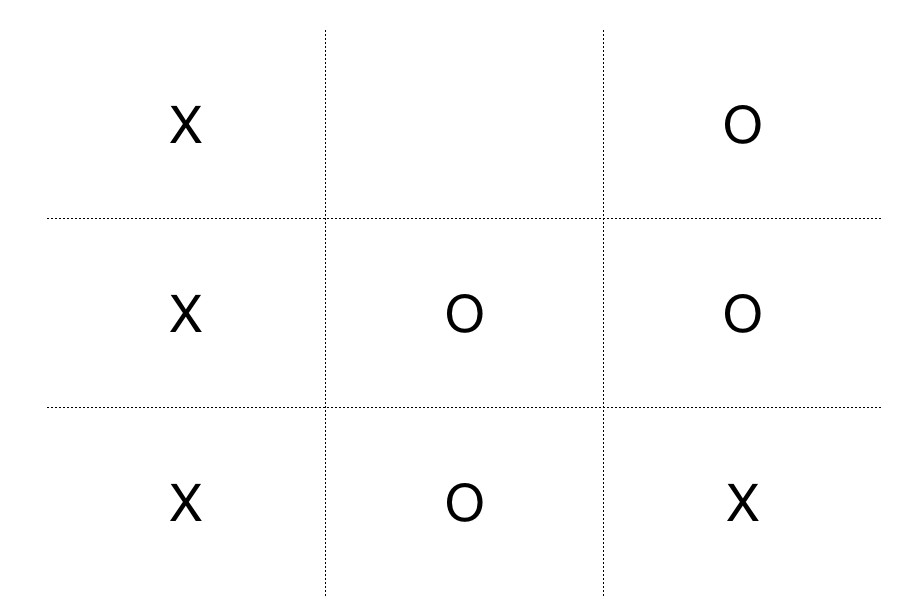
\includegraphics [scale=0.22] {ttt_1.png}
	\caption{Stan gry dla ciągu (2, 0, 1, 2, 1, 2,  2, 1, 1.0)}
	\label{Rys9}
\end{figure}


Kolejny wpis w tabeli, to ciąg $1, 2, 2, 2, 1, 1, 0, 1, 2, 0.75$. Pierwsze 9 cyfr przedstawia stan gry zobrazowany na rysunku \ref{Rys10}. Jak widać, niezależnie od ruchu gracza reprezentującego system (gracz posługujący się kółkiem), gra zakończy się remisem. Stąd wartość $q$ w tym przypadku jest równa $0.75$. \\

\begin{figure}[h!]
	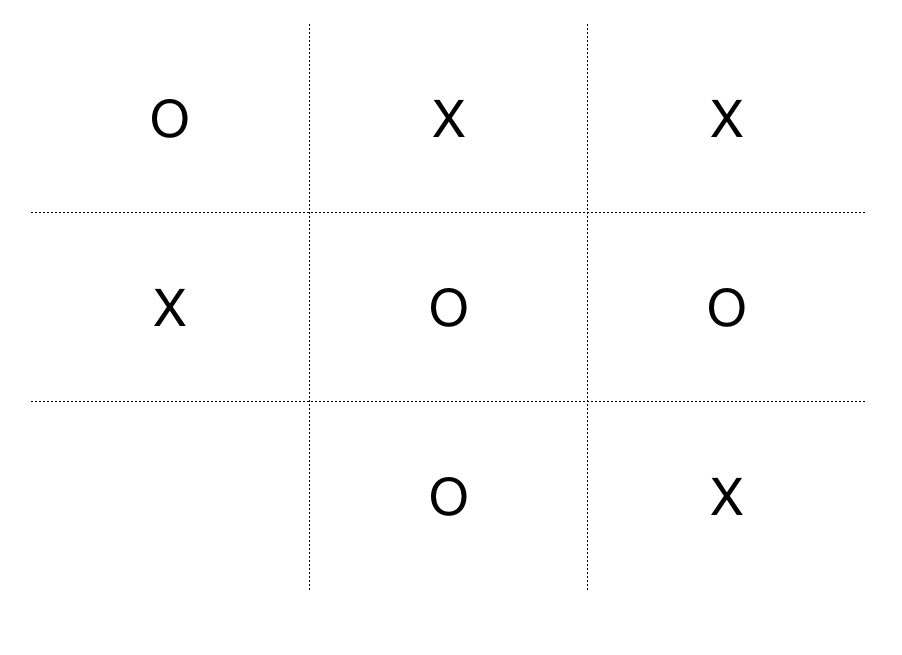
\includegraphics [scale=0.22] {ttt_2.png}
	\caption{Stan grdy dla ciągu (1, 2, 2, 2, 1, 1, 0, 1, 2, 0.75)}
	\label{Rys10}
\end{figure}

Kolejny wiersz, to ciąg $2, 2, 1, 2,  2, 1, 1, 0, 0, -1$ (rysunek \ref{Rys11}), jak łatwo zauważyć przedstawia sytuację, w której  ruch należy do gracza systemowego (kółko lub cyfra 1) i gracz ten może z łatwością wygryać uzyskując trzy ,,kółka'' na prawej skrajnej kolumnie. Stąd wartość $q$ w tym przypadku jest równa $-1$.\\

\begin{figure}[H]
	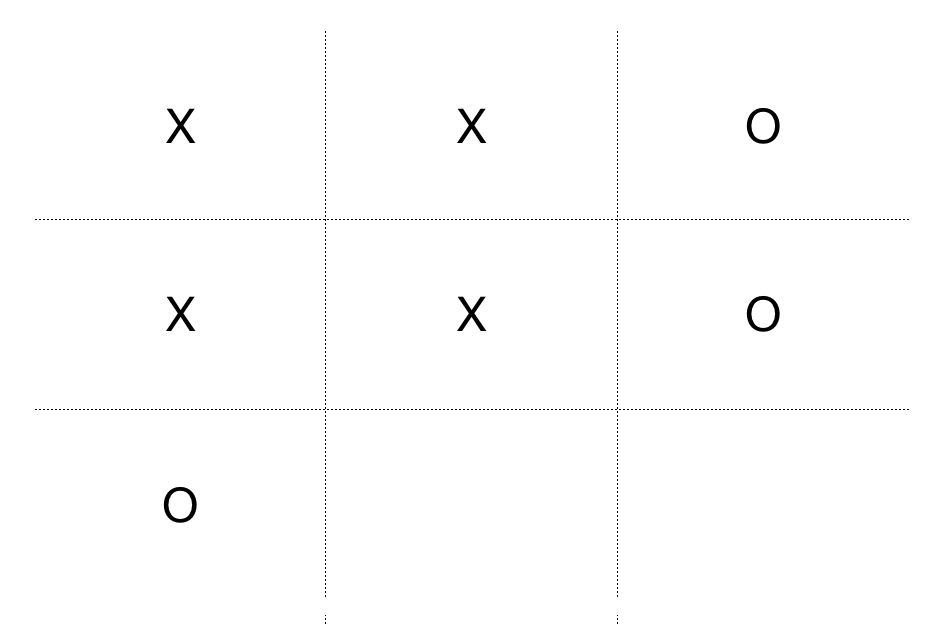
\includegraphics [scale=0.22] {ttt_3.png}
	\caption{Stan gry dla ciągu (2, 2, 1, 2,  2, 1, 1, 0, 0, -1)}
	\label{Rys11}
\end{figure}

Czwarty przykład odpowiadający ciągowi $2, 0, 0, 1, 2, 2, 0, 0, 0, 0.418681257165$  zilustrowany na rysunku \ref{Rys12} to gra w stanie jeszcze mało zaawansowanym, w którym obaj gracze mają szansę wygrać lub przegrać. W tym przypadku wyczuona wartość $q$ wynosi około $0.42$, co wskazywałoby, że jest to relatywnie korzystna sytuacja dla agenta grającego ,,krzyżykiem''.

\begin{figure}[h!]
	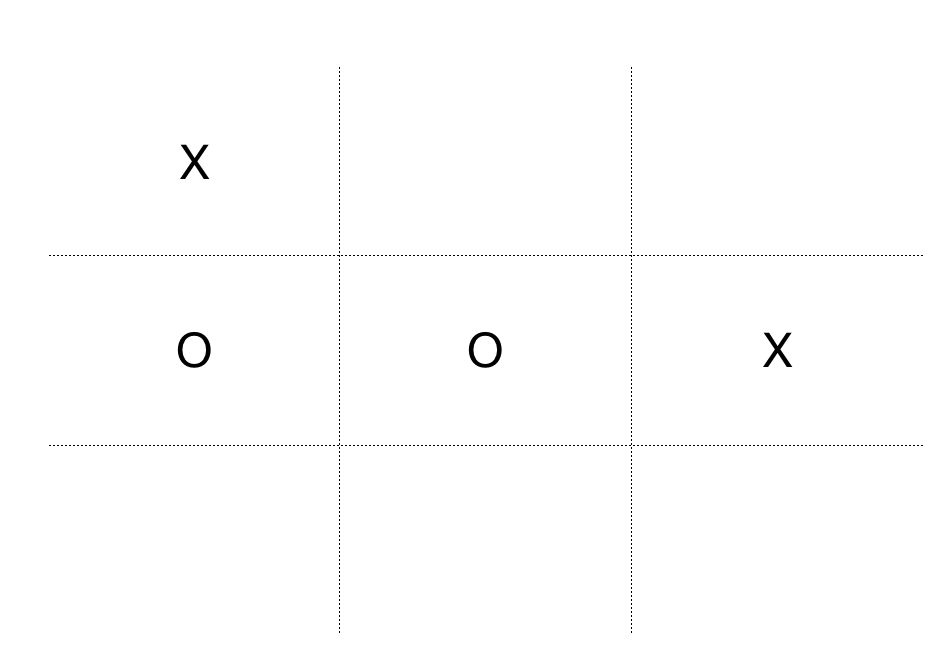
\includegraphics [scale=0.22] {ttt_4.png}
	\caption{Stan gry ciągu dla (2, 0, 0, 1, 2, 2, 0, 0, 0, 0.418681257165)}
	\label{Rys12}
\end{figure}


Ostatni przykład, to ciąg $ 2, 0, 2, 2, 1, 0, 1, 1, 0, -0.0186631984604$ Wartość $q$ lekko ujemna wskazuje na neutralność tego stanu. Ten przykład jest ciekawy i pokazuje słabość algorytmu. System może w kolejnym ruchu wygrać grę. Pamiętajmy jednak, że algorytm uczył się grając z graczem losowym, który nie koniecznie wykorzysta możliwość wygrania i z tego stanu możliwe jest nadal zwycięstwo agenta (ale remis już nie). Przypuszczalnie dlatego wartość oczekiwana przyszłych nagród jest bliska zero. Gdyby uczyć algorytm poprzez grę tylko i wyłącznie z idealnym graczem, to najprawdopodobniej ten stan (po przetrenowaniu) miałby wartość bliższą $-1$.
\begin{figure}[h!]
	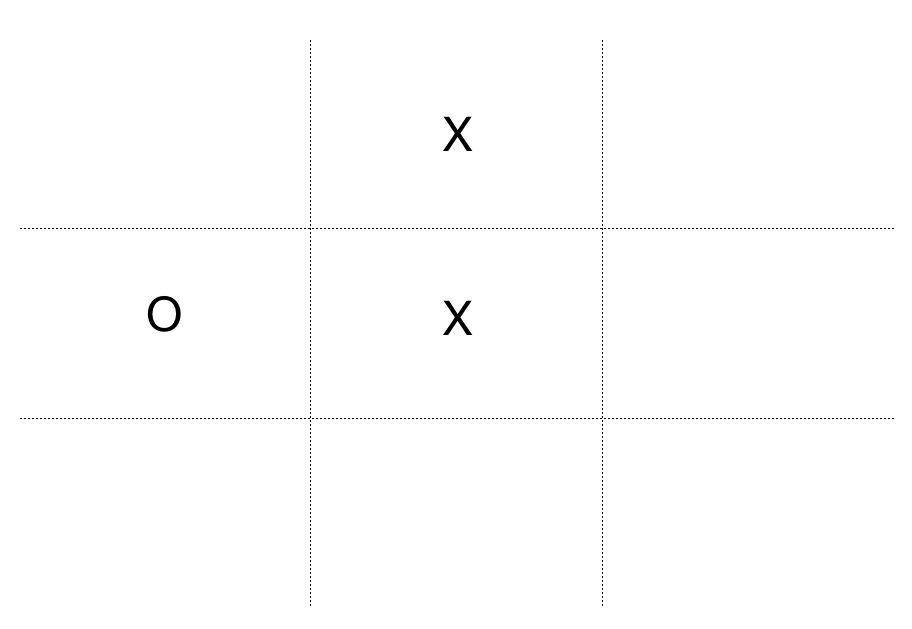
\includegraphics [scale=0.22] {ttt_5.png}
	\caption{Stan gry dla ciągu (2, 0, 2, 2, 1, 0, 1, 1, 0, -0.0186631984604) }
	\label{Rys13}
\end{figure}

Mając wszystkie niezbędne elementy można przejść do bezpośredniego zdefiniowania algorytmu:


\begin{enumerate}
	\item{Inicjuj pusty zbiór z wartościami $q_{s}$}
	\item{Ustaw parametry $\alpha$ i $\gamma$ z przedziału $[0, 1]$}
	\item{Graj n razy z systemem w kółko i krzyzyk:}
	\begin{enumerate}
		\item{Jeżeli jest ruch agenta, a plansza jest w stanie $s-1$:}
		\begin{enumerate}
			\item{Dla każdego legalnego ruchu prowadzącego z $s-1$ do $s$  sprawdź wartość $q_{s}$ w zbiorze, a jeżeli nie ma zbiorze wartości $q_{s}$, to przyjmij $q_{s}=0$.}
			\item{Wybierz ten ruch $\tilde{s}$, dla którego $q_{\tilde{s}} =\max_{s} q_{s}$. Jeżeli jest kilka takich ruchów, to wybierz jeden losowo.}
			\item{Połóż $q_{s-1} = q_{s-1} + \alpha(R(\tilde{s}) + \gamma  q_{\tilde{s}} - q_{s-1} )$ }
			\item{Zapisz nową wartość $q_{s-1}$ w zbiorze. Jeżeli wartość już istniała w zbiorze, to nadpisz.}
		\end{enumerate}
	\end{enumerate}
\end{enumerate}

Popatrzmy  teraz na wyniki uczenia. Zaczynając od pustego zbioru $q_{s}$ rozegrano po 100 partii z graczem losowym i z graczem stosującym minmax. Dodatkowo po każdej grze ,,opróżniany'' jest zbiór $q_{s}$ tak żeby algorytm na razie niczego nie uczył się,   po to, żeby mieć później punkt odniesienia przy sprawdzaniu postępów w uczeniu się gry. W poniżyszych przykładach agent jest zawsze graczem korzystającym z ,,kółka", a system jest reprezentowany przez ,,krzyżyk". \\

W 100 grach rozegranych z graczem losowym otrzymałem wyniki jak na rysunku \ref{Rys14}.\\
\begin{figure}[h!]
	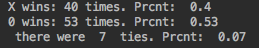
\includegraphics [scale=0.7]{Qtable_vs_Rnd_untrained.png}
	\caption{Wynik 100 gier z graczem losowym(X) przed uczeniem algorytmu}
	\label{Rys14}
\end{figure}
Jak widać agent jest nieznacznie lepszy od systemu, ale praktycznie w granicach losowego wahania.\\

Natomiast 100 gier rozegranych z graczem minimax (zobacz rysunek \ref{Rys15}) dało 10 remisów i 90 przegranych agenta\\
\begin{figure}[h!]
	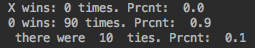
\includegraphics [scale=0.7]{QTable_vs_Minimax_untrained.png}
	\caption{Wynik 100 gier z gracem minimax (X) przed uczeniem algorytmu}
	\label{Rys15}
\end{figure}

Po przeuczeniu algorytmu na 20 000 grach z graczem losowym, zbiór $q_{s}$ ma 775 rekordów (tyle różnych stanów  agent napotkał podczas rozegranych gier), natomiast wyniki dla 100 gier, przedstawione na rysunku \ref{Rys16} teraz wyglądają już znacznie lepiej.\\

\begin{figure}[h!]
	\includegraphics [scale=0.7]{Qtable_vs_Rnd_trained.png}
	\caption{Wynik 100 gier z graczem losowym(X) po przetrenowaniu algorytmu}
	\label{Rys16}
\end{figure}


Z graczem losowym, wytrenowany agent przegrywa tylko w 3\%, ma 76\% wygranych i 21\% remisów. Grając z tak wytrenowanym agentem można odczuć, że gra całkiem dobrze, ale jeszcze czasami potrafi wykonać poważny błąd. Nie ma natomiast prawie żadnej poprawy jeżeli chodzi o liczbę remisów (bo wygrać się nie da) z systemem grającym strategią minimax, co widać na rysunku \ref{Rys17}. \\

\begin{figure}[h!]
	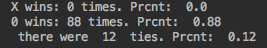
\includegraphics [scale=0.7]{QTable_vs_Minimax_trained.png}
	\caption{Wynik 100 gier z graczem minimax (O) po przetrenowaniu algorytmu}
	\label{Rys17}
\end{figure}

Nasuwa się oczywiście pytanie, czy przetrenowanie algorytmu na grach z systemem grającym strategią minimax poprawiłoby tą statystykę?. Na rysunku \ref{Rys18} przedstawione zostały wyniki algorytmu po dodatkowych 10 000 grach z systemem grającym strategią minimax.\\

\begin{figure}[h!]
	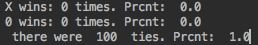
\includegraphics [scale=0.7]{QTable_vs_Minimax_trained_d.png}
	\caption{Wynik 100 gier z graczem minimax (O) po przetrenowaniu algorytmu}
	\label{Rys18}
\end{figure}

A więc trenowanie algorytmu na systemie grającym strategią minimax odniosło skutki.  Agentowi udało się 100 razy na 100 gier zremisować z graczem grającym według minimax. Warto jeszcze sprawdzić, czy po tym trenowaniu algorytm nie odnotuje gorszych wyników grając z graczem losowym. Wyniki zamieszczono na rysunku \ref{Rys19}.\\

\begin{figure}[h!]
	\includegraphics [scale=0.7]{QTable_vs_Rnd_trained_d.png}
	\caption{Wynik 100 gier z graczem losowym(X) po dodatkowym przetrenowaniu algorytmu z graczem minimax}
	\label{Rys19}
\end{figure}

Jak widać wyniki uległy nawet poprawie. Agent po dodatkowym trenowaniu wygrywa w 84\%, przegrywa w 2\% i w 14\% remisuje. Należy jednak zaznaczyć, że takie trenowanie algorytmu z systemem, który gra zgodnie ze strategią minimax, nie jest zupełnie zgodne z pierwotną ideą, żeby algorytm nauczył się grać w kółko i krzyżyk bez żadnych dodatkowych informacji, w tym bez możliwości uczenia się przez grę z optymalną strategią. \\

Na koniec warto jeszcze dodać, że po takim podwójnym trenowaniu, czysto subiektywne odczucie jest takie, że algorytm gra w sposób zbliżony do człowieka. Rzadko popełnia oczywiste błędy, a chwila nie uwagi kończy się zazwyczaj przegraną. 

 
\chapter{Sieć neuronowa grająca w kółko i krzyżyk }\label{r:Siec}

\section{Sieci neuronowe}
Metoda opisana w poprzednim rozdziale ma jedną zasadniczą wadę. Dla gier o znacznie większej liczbie możliwych kombinacji plansz, zbiory z wartościami $q_{s}$ stają się ogromne. O ile jeszcze samo zapisanie takiego zbioru, zważywszy na szybki rozwój elektronicznych nośników danych, mógłby być możliwy, to już przeszukiwanie przed każdym ruchem zbioru w celu wyłonienie tego, który maksymalizuje $q_{s}$ jest absolutnie nie wykonalne. Alternatywą do przechowywania wartości $q_{s}$ w tabeli lub pliku, może być wytrenowanie sieci neuronowej w taki sposób, żeby estymowała funkcję $s\rightarrow q_{s}$\\

Sieć neuronowa składa się z neuronów. Natomiast jeden neuron ma określoną liczbę $n$ danych wejściowych, odpowiadającą tej ilości liczbę wag $w_{i}, 1 < i\leq n+1$, (o jeden więcej niż ilość danych wejściowych) przy czym wprowadza się 
oznaczenie  $b=w_{n+1}$ (wyraz stały)  , oraz zadaną funkcję aktywacji $f:\mathbf{R}\rightarrow\mathbf{R}$.  Załóżmy, że dane wejściowe to $x_{1}, x_{2},...,x_{n}$.  Neuron wylicza sumę ważoną tych danych powiększoną o wyraz stały $w_{n+1}$ i zwraca wartość funkcji aktywacji z tej sumy :

%$$f(\sum_{i=1}^{n}w_{i}x_{i} +b)$$
\begin{figure}[h!]
	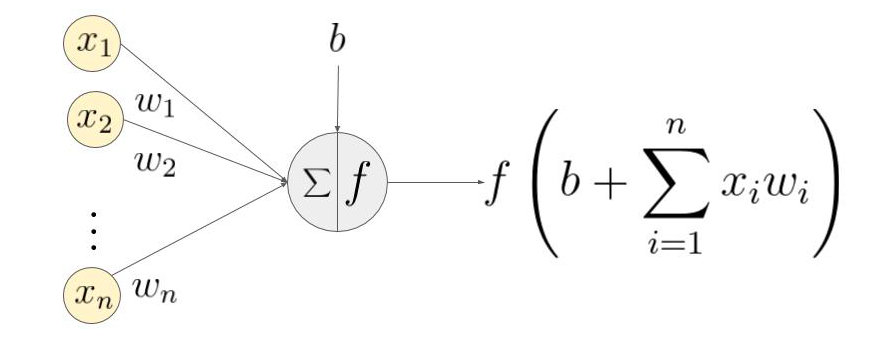
\includegraphics [scale=0.2]{neuron.png}
	\caption{Zasada działania neuronu}
	\label{Rys20}
\end{figure}


Funkcja aktywacji może być w zasadzie dowolna. Ze względu na łatwość ,,uczenia" sieci neuronowej, o czym za chwilę, warto stosować funkcje różniczkowalne (ewentualnie różniczkowalne poza kilkoma punktmai) i monotoniczne. Najczęściej stosuje się takie funkcje jak sigmoid, tanges hiporbeloczny, relu, czy softplus.  Poniżej definicja i wykres (rysunek \ref{Rys21}) funkcji sigmoid - najbardziej klasycznego przykładu funkcji aktywacji.

$$sigmoid(x) = \frac{1}{1-e^{-x}}$$
\begin{figure}[h!]
	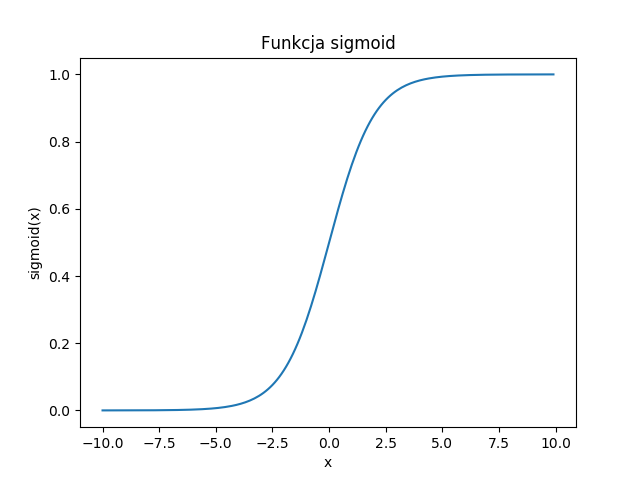
\includegraphics [scale=0.5]{sigmoid.png}
	\caption{Wykres funkcji aktywacji - sigmoid}
	\label{Rys21}
\end{figure}


Sieć neuronowa składa się, jak nazwa wskazuje z wielu neuronów, ułożonych w warstwy. Pierwsza warstwa, to warstwa wejściowa danych. Dane z wejściowe są przekazywane neuronom w w drugiej warstwie z neuronami. Każdy neuron ma swój zestaw wag, które służą do utworzenia kombinacji liniowej z danych wejściowych, po czym neuron zwraca wartości funkcji aktywacji na tej kombinacji liniowej. Wartości zwracane przez neurony w drugiej warstwie są z kolei przekazywane do trzeciej warstwy z neuronami, tak jak dane wejściowe zostały przekazane do drugiej warstwy (pierwszej z neuronami).  Wartości obliczone na ostatniej warstwie z neuronami, to są wartości ostatecznie zwracane przez sieć. 

\begin{figure}[h!]
	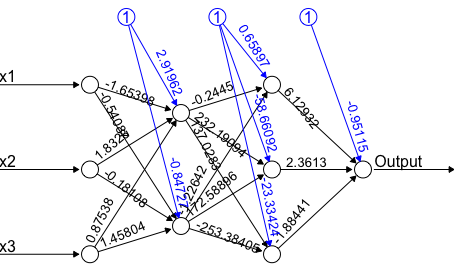
\includegraphics [scale=0.7]{nn_example.png}
	\caption{Przykład sieci neuronwej wygenerewany w R}
	\label{Rys22}
\end{figure}

Powyżej, rysunek \ref{Rys22} przedstawia przykładową sieć, która ma trzy wartości wejściowe, a następnie warstwę 2 neuronów, warstwę 3 neuronów i ostatnią warstwę wyjściową składającą się z jednego neuronu. Wartości na strzałką pokazuję wartości wag neuronu, do którego prowadzi strzałka. Dodatkowo, na niebiesko zaznaczono wartości stałe ($b$) dla poszczególnych neuronów. Przy tworzeniu sieci neuronowej, ważne jest, żeby ilość wag dla każdego neuronu w k-tej warstwie, była równa ilości neuronów (lub danych wejściowych) w k-1-ej warstwie (plus dodatkowo wyraz stały). W przeciwnym razie nie uda się uwzględnić wszystkich wartości z k-1 warstwy w kombinacji liniowej.  \\
 
Podsumowując można powiedzieć, że siecią neuronową, o zadanej strukturze, jest funkcja $\mathbf{\mathcal{N}}$, której argumenty, to zbiór wartości wejściowych $x_{1},...,x_{n}$ oraz zbiór wszystkich wag $\mathbf{W}$ i zbiór wszystkich wyrazów stałych $\mathbf{b}$, która zwraca wektor wartości $y_{1},...,y_{m}$ o wymiarze równym ilości neuronów w ostatniej warstwie.

$$\mathcal{N}(x_{1},...,x_{n}, \mathbf{W}, \mathbf{b}) = (y_{1},...,y_{m})$$

Argumenty $\mathbf{W}$  i $\mathbf{b}$ można traktować jak parametry funkcji $\mathbf{\mathcal{N}}$. Zasdaniczym celem jest tak zmieniać te parametry, żeby sieć neuronowa $\mathbf{\mathcal{N}}$ przybliżała nam jakąś rzeczywistą, obserwowalną, ale nieznaną funkcję $\Phi$: 
$$ (x_{1},...,x_{n})\stackrel{\Phi}{\rightarrow}(y_{1},...,y_{m})$$

Poniżej przedstawiony został zarys klasycznej metody uczenia sieci neuronowych (czyli de facto dostrajania wag   $\mathbf{W}$  i $\mathbf{b}$ na podstawie danych danych) bazujący na pierwszych rozdzaiałach \cite{nn}.\\
 
Po pierwsze, skoro celem jest przybliżanie funkcji $\Phi$ siecią neuronową $\mathbf{\mathcal{N}}$, to potrzebna jest jakaś miara skuteczności takiego przybliżenia.  Załóżmy, że mam k-elementowy zbiór danych (treningowych) $\mathbf{X}$ i dla każdego $x_{1},...,x_{n}\in\mathbf{X}$ obserwujemy $\Phi(x_{1},...,x_{n})$ oraz $\mathbf{\mathcal{N}}(x_{1},...,x_{n}, \mathbf{W}, \mathbf{b})$. Jak w tym przypadku określić skuteczność przybliżania $\Phi$ za pomocą sieci $\mathbf{W}, \mathbf{b}$ na zbiorze $\mathbf{X}$? W literaturze można spotkać wiele metod, ale chyba najbardziej naturalną jest średnio kwadratowa funkcja straty (kosztu) , którą zapiszemy jako funkcję parametrów $\mathbf{W}$ i $\mathbf{b}$.
 
\begin{equation}
	\label{Cost_function}
	C(\mathbf{W}, \mathbf{b}) = \frac{1}{2k}\sum_{(x_{1},...,x_{n})\in\mathbf{X}}{\norm{\Phi(x_{1},...x_{n}) - \mathbf{\mathcal{N}}(x_{1},...,x_{n}, \mathbf{W}, \mathbf{b} )} } ^{2}
\end{equation}
 
 
Norma występującą w powyższym wyrażeniu, to zwykła odległość euklidesowa w przestrzeni $\mathbf{R^{d}}$. Zauważmy, że jeżeli ustalimy zbiór testowy $\mathbf{X}$ i zbiór obserwacji $\Phi(\mathbf{X})$, to powyższą funkcję kosztu możemy rozpatrywać jako funkcję parametrów sieci neuronowej $\mathbf{\mathcal{N}}$. Przy takim podejściu, znalezienie wag $\mathbf{W}$ i $\mathbf{b}$, dla których sieć $\mathbf{\mathcal{N}}$ będzie najlepiej przybliżać funkcję $\Phi$ sprowadza się do znalezienia minimum funkcji $C(\mathbf{W}, \mathbf{b}):\mathbf{R^{d}}\rightarrow\mathbf{R}$, dla pewnej liczby naturalnej d.  Dla uproszczenia zapisu przyjmijmy, żę $v:=(\mathbf{W}, \mathbf{b})$. Czyli funkcja kosztu C będzie funkcją zmiennej $v\in\mathbf{R^{d}}$. Z rachunku różniczkowego wiadomo, że:
 
\begin{equation}
	\label{nn_u}
	\Delta C = \nabla C \cdot \Delta v
\end{equation}
 
W powyższym równaniu symbol $(\cdot)$ oznacza iloczyn skalarny wektorów. Natomiast $\nabla C$ to jest gradient funkcji C, czyli $\nabla C = (\frac{\delta C}{\delta v_{1}},...,\frac{\delta C}{\delta v_{d}} )$. Zwróćmy uwagę, że $\Delta C$ jest zwykłym skalarem. Jeżeli ustalimy sobie $v$ i pewną małą wartość $\eta>0$, to możemy położyć:
$$v' = v + \eta\nabla C(v), $$
$$ \Delta v = v - v'$$
 
i wstawimy do (\ref{nn_u}), to otrzymamy:
$$\Delta C = \nabla C\cdot (v - v)' = -\eta \nabla C\cdot\nabla C = -\eta\norm{\nabla C}^{2} < 0$$
 
Jeżeli więc będziemy zmieniać komplet wag zgodnie ze wzorem:
$$v':=v+\eta\nabla C(v),$$
to będziemy zmniejszać wartość $\Delta C$, co oznacza, że będziemy podążali w kierunku minimum funkcji C. Ta metoda znana jest w literaturze (np. \cite{nn}) jako ,,\textit{gradient descent}''. Ważnym parametrem w tej metodzie jest $\eta$, często nazywana w angielskojęzycznej literaturze \textit{learning rate}. Jeżeli $\eta$ jest duże, to potrzeba będzie mniej kroków na odnalezienie lokalnego minimum, ale zagrożenie jest takie, że zmieniając wagi będziemy ,,przeskakiwać'' nad minimum niewiele zbliżając się do niego. Z drugiej strony, zbyt małe $\eta$ może skutkować koniecznością wykonania bardzo wielu kroków w celu odnalezienia minimum.\\

Jeżeli liczba d jest duża, to analityczne szukanie punktów, w których zerują się wszystkie pochodne cząstkowe byłoby kosztowne obliczeniowo jeżeli nie niewykonalne. W praktyce często przyjmuje się inne podejście; odmianę tej metody znaną jako  ,,\textit{stochastic gradient descent}'' (dalej SGD), która różni się tym, że funkcję kosztu $C$ (\ref{Cost_function}) wyliczamy na podstawie losowo wybranego podzbioru ze zbioru testowego $\mathbf{X}$ i odpowiadających obserwacji $\Phi(\mathbf{X})$. Dla jednego zbioru obserwacji $\mathbf{X}$ wielokrotnie losować podzbioru, obliczać $\nabla C$ zdefiniowanego dla wylosowanego podzbioru i aktualizować wagi $v$. W literaturze można przeczytać, że taka metoda pozwala na skuteczne dobranie wag. Skrajny przypadek metody STD, to branie tylko jednej obserwacji do wyliczenia funkcji kosztu.\\
 
Reasumując, jeżeli potrafilibyśmy policzyć gradient $\nabla C$ dla funkcji kosztu, to mamy przepis na to jak zmieniać wagi $\mathbf{W}$ i wartosci stałe $\mathbf{b}$, czyli parametry sieci $\mathcal{N}$, w sposób, który gwarantuje nam zmniejszanie nam wartości funkcji kosztu, a więc poprawiający przybliżenie. Tutaj z pomocą przychodzi algorytm propagacji wstecznej (z ang. \textit{,,backpropagation algorithm ``}. Algorytm propagacji wstecznej, jest podstawowym algorytmem, który w połączeniu z powyższymi rozważaniami o tym jak zmieniać wagi sieci, pozwala na skuteczne trenowania sieci. W wielkim skrócie, algorytm propagacji wstecznej sprawdza się do wliczenia wartości aktywacji na każdym neuronie, a następnie - idąc od ostatniej warstwy wyjściowej aż d pierwszej warstwy (stąd zapewne nazwa propagacji wstecznej) obliczenia błędów sieci i modyfikowanie wag na każdym poziomie. Dokładny opis algorytm, jak również dowód poprawności algorytmu, jest dostępny w niemal każdym opracowaniu traktującym o podstawach sieci neuronowych. Ponieważ niniejsza praca raczej ma się koncentrować na praktycznych aspektach uczenia sieci, to opis algorytmu zostaje pominięty.

\section{Podejście I - nieudane}

Biorąc pod uwagę, że trenowanie algorytmu opisanego w poprzednim rozdziale dało całkiem dobre rezultaty, to naturalnym pomysłem było zastąpienie tabeli przypisujących stanom $s$ wartości $q_{s}$ siecią neuronową i pozostawienie pozostałych elementów niezmienionych. W rezultacie otrzymuje się taki algorytm:

\begin{enumerate}
	\item{Inicjuj sieć neuronową, która przyjmuje na wejściu 9 wartości i zwraca na wyjściu 1 wartość -  $q_{s}$}
	\item{Ustaw parametry $\alpha$ i $\gamma$ z przedziału $[0, 1]$}
	\item{Graj n razy z systemem w kółko i krzyzyk:}
	\begin{enumerate}
		\item{Jeżeli jest ruch agenta, a plansza jest w stanie $s-1$:}
		\begin{enumerate}
			\item{Dla każdego legalnego ruchu prowadzącego z $s-1$ do $s$  sprawdź zwracaną przez sieć neruonową wartość $q_{s}$}
			\item{Wybierz ten ruch $\tilde{s}$, dla którego $q_{\tilde{s}} =\max_{s} q_{s}$. Jeżeli jest kilka takich ruchów, to wybierz jeden losowo.}
			\item{Połóż $q_{s-1} = q_{s} + \alpha(R(\tilde{s}) + \gamma  q_{\tilde{s}} )$, gdzie $R(\tilde{s})$ jest nagrodą po ruchu $\tilde{s}$. }
			\item{Przetrenuj sieć na jednoelementowym zbiorze \{$s-1$, $q_{s-1}$\} }.
		\end{enumerate}
	\end{enumerate}
\end{enumerate}

Pozostaje jeszcze kwestia ustalenia topologii sieci i tego jaka będzie funkcja aktywacji. Kółko i krzyżyk nie jest skomplikowaną grą, stąd decyzja o sieci z jedną warstwą ukrytą. Warstwa wejściowa, to oczywiście 9 pozycji odpowiadających dziewięciu polom na planszy. Warstwa wyjściowa, to jedna pozycja zwracającą $q_{s}$ dla stanu reprezentowanego przez dane wejściowe. Przy czym podobnie jak w poprzednim rozdziale, dane wejściowe reprezentują stan gry po ruchu agenta. Ilość neuronów w warstwie ukrytej wybrano poniekąd arbitralnie na $27$. Ze względu na symetrię miała to to być  wielokrotność (jednak nie za duża) ilości danych wejściowych. 

\begin{figure}[h!]
	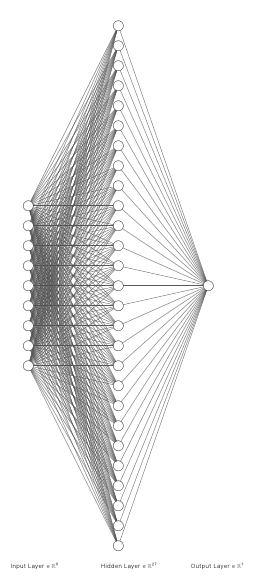
\includegraphics [scale=0.5]{nn_1pod.png}
	\caption{Topologia sieci w I podejściu}
	\label{Rys23}
\end{figure}


 Na koniec jeszcze pozostaje ustalenie funkcja aktywacji. Ponieważ $q_{s}$ reprezentuje wartość oczekiwaną przyszłych nagród, to ważne jest, żeby funkcja aktywacji miała zbiór wartości obejmujący zakres możliwych wartości przyszłych nagród. W poprzednim rozdziale, przyjęti takie wartości:

\begin{enumerate}
	\item{-1 w przypadku przegranej}
	\item{0.75 w przypadku remisu }
	\item{1 w przypadku wygranej}
	\item{0 dla każdego innego stanu gry}
\end{enumerate}

Ponieważ wygrana, remis, lub przegrana w grze może się zdarzyć tylko raz, to wartość oczekiwana przyszłych nagród, będzie w zakresie  $[-1,1]$ i  stąd dobrze mieć funkcję aktywacji obejmującą ten przedział. Dobrym kandydatem byłaby funkcja $\tanh$, czyli tangens hiberboliczny, którego zbiór wartości to właśnie przedział $[-1,1]$. Problem jednak jest taki, że jeżeli funkcja aktywacji ,,wypłaszcza" się dla dużych argumentów, to jej pochodna jest bliska zeru, co z kolei przekłada się na to, że algorytm propagacji wstecznej (czyli ten, który liczy gradient funkcji kosztu) szacuje pochodne na bliskie zeru i cały algorytm uczenia sieci neuronowej prawie nie aktualizuje wag $\mathbf{W}, \mathbf{b}$. Chcąc uniknąć takiego efektu ,,saturacji", za funkcję aktywacji przyjęto $f(x) = 2\tanh(x)$. Dla porządku, podano ponizej definicję funkcję tangens hiperboliczny i joraz przedstawiono jej wykres na rysunku \ref{Rys24}.

\begin{figure}[h!]
	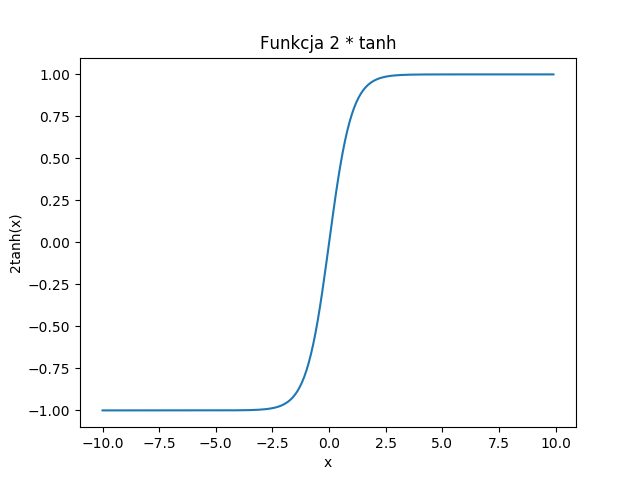
\includegraphics [scale=0.5]{tanh.png}
	\caption{Tangens hiperboliczny przemnożony przez 2}
	\label{Rys24}
\end{figure}

\begin{equation}
	\tanh(x) = \frac{e^{2x} - 1}{e^{2x} + 1}
\end{equation}

Niestety takie proste zastąpienie tabeli przechowującej wartości $q_{s}$ przez sieć neuronową, która miałaby w podobny sposób, po każdym ruchu poprawić swoje oszacowanie $q_{s}$ nie zdało egzaminu. Po długotrwałym trenowaniu (20 000 gier z graczem losowym) taka sieć potrafi wygrywać z graczem losowym w około 60\%-70\% przypadków, i w subiektywnym odczuciu gra zdecydowanie gorzej od człowieka.  Poniżej (rysunek \ref{Rys25}) wynik 100 rozegranych gier na przetrenowanej sieci:

\begin{figure}[h!]
	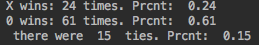
\includegraphics [scale=0.7]{nn_I_tanh.png}
	\caption{}
	\label{Rys25}
\end{figure}

Eksperymenty z większą liczbą neuronów w warstwie ukrytej, jak również z dwiema warstwami ukrytymi, oraz z innymi funkcjami aktywacji, kończyły się ale zawsze z podobnym, niezadawalającym efektem. Najlepsze wyniki jakie udało się uzyskać, to około 75\% wygranych gier z graczem losowym. Wyniki takie uzyskano używając funkcji aktywacji $softplus$, która definiuje się jako  $f(x) = ln(1+e^{x})$ Ta funkcja aktywacji przyjmuje wartości z przedziału $[0,+\infty]$  (jest to wygładzona wersja innej popularnej funkcji aktywacji -  ReLu), stąd konieczna była zmiana wartości nagród. W tym przypadku przyjąłem:

\begin{enumerate}
	\item{0.5 w przypadku przegranej}
	\item{75 w przypadku remisu }
	\item{100 w przypadku wygranej}
	\item{1 dla każdego innego stanu gry}
\end{enumerate}

Poniżej (rysunek \ref{Rys26}) )wynik rozegranych 100 gier z graczem losowym po przetrenowaniu na 20 000 gier.

\begin{figure}[h!]
	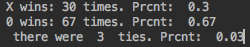
\includegraphics [scale=0.7]{nn_I_softplus.png}
	\caption{}
	\label{Rys26}
\end{figure}

Jak widać, sieć gra statystycznie nieco lepiej od gracza losowego, czyli algorytm ,,czegoś" się nauczył, ale przy tak prostej grze jak kółko i krzyżyk można by się spodziewać znacznie lepszych rezutlatów. Należy jeszcze dodać, że dla wszystkich wypróbowanych kombinacji sieci, po przetrenowaniu, miały procent remisów z graczem minimax na poziomie od 0\% do 5\%.


\section{Podejście II - bardziej udane}

Dlaczego sieci z poprzedniej sekcji nie udało się dobrze nauczyć grać w kółko i krzyżyk? Trudno oczywiście o kategoryczną odpowiedzieć na to pytanie, ale można postawić hipotezę, że problem leży w tym, że sieć uczy się po każdym ruchu na jedno-elementowym zbiorze treningowym. Takie rozwiązanie ma zasadniczą wadę. Większość ruchów skutkuje nagrodą równą zero. Dopiero ostatni ruch w grze kończy się inną wartością nagrody. Sieć natomiast modyfikuje wagi po każdym ruchu i używa tych zmodyfikowanych wag do dalszej gry i dalszego uczenia.  To może może powodować, że wielokrotnie modyfikując wagi dla ruchów z zerową nagrodą sieć ,,zapomina" wagi, które pozwalały wygrać. Lepszym podejściem byłoby rozegranie wielu gier (wielu ruchów) i przekazanie sieci do trenowania jednego dużego zbioru danych. W tej częśc takie podejście zostało wypróbowane. Pomysł został zaczerpnięty z pracy magisterskiej złożonej na uniwersytecie technicznym w Monachium \cite{TUM}.\\

Dodatkowo, żeby wyeliminować ewentualny problem zbyt małej sieci, zmieniono jej topologię dodając jedną warstwę ukrytą. Ostatecznie sieć ma strukturę typu 9-54-27-1, czyli zwiera dwie warstwy ukryte po 54 i 27 neuronów odpowiednio.  Za funkcję aktywacji przyjęto tangens hiperboliczny, który przyjmuje wartości z przedziału $[-1,1$. Nagrody, czy odpowiedź systemu, ustalono z uwagą żeby być daleko od ekstremalnych wartości funkcji aktywacji:

\begin{enumerate}
	\item{-0.8 w przypadku przegranej}
	\item{0.5 w przypadku remisu }
	\item{0.8 w przypadku wygranej}
	\item{0 dla każdego innego stanu gry}
\end{enumerate}

Sam proces uczenia sieci wygląda teraz następująco. Ustala się arbitralnie wielkość zbioru do uczenia (w literaturze odpowiednik pojęcia \textit{batch size}) np. na 2500. Następnie rozgrywane jest tyle gier, żeby zebrać 2500 obserwacji. Przy czym jedną obserwacją będzie teraz wektor przechowujący stan planszy po ruchu agenta (gracza odpowiadającego sieci neuronowej), wartość $q_{s}$ czyli zwróconą przez sieć przyszłą oczekiwaną wartość nagród  oraz rzeczywistą nagrodę $R$  jaką system zwrócił po swoim ruchu lub po zakończeniu gry, jeżeli ruch agenta był ostatnim ruchem. Najlepiej zobaczyć jak to wygląda na przykładzie.\\

Pierwsze 9 pozycji odwzorowuje planszę gry. Zero odpowiada pustemu polu, jedynka to pole zajęte przez system (w tym wypadku gracz losowy), a dwójka to pole zajęte przez agenta.
W poniższym (rysunkek \ref{Rys27}) przykładzie zaczyna agent, stawia krzyżyk (dwójkę) na środkowym polu. Na 10 pozycji  - wartość 0.642  - znajduje się oczekiwana wartość przyszłych nagród zwrócona przez sieć. Następnie jest oczekiwanie na ruch systemu, chyba że to jest ostatni ruch w grze, i dopiero po tym ruchu systemu dopisujemy nagrodę jaką otrzyma agent. W tym wypadku będzie to zero, bo gra jeszcze się nie skończy.

 
\begin{figure}[h!]
	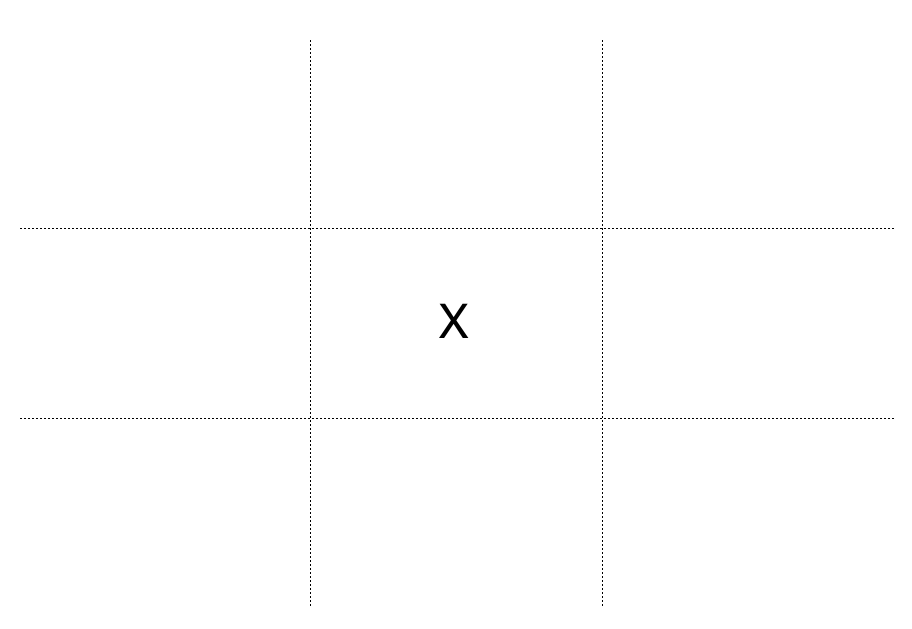
\includegraphics [scale=0.2] {ttt_6.png}
	\caption{}
	\label{Rys27}
\end{figure}
$\text{Obserwacja po pierwszym ruchu:  }[0, 0, 0, 0, 2, 0, 0, 0, 0, 0.642, 0]$\\

 Następnie system stawia swoje kółko w na pozycji $2,1$, czyli w pierwszej kolumnie i w drugim rzędzie. Ten stan planszy nie zostanie zapisany, bo interesujące są tylko stany po ruchu agenta. Jednak po ruchu systemu sprawdza się jaka jest nagroda agenta i tym samym, dopiero po tym ruchu systemu mamy w pełni uzupełnioną pierwszą obserwację. Kolejny, trzeci ruch w grze, należy do agenta i ten wybiera (sprawdzając jaki ruch będzie skutkował maksymalną oczekiwaną nagroda $q_{s}$) pozycję $1,2$:
 
\begin{figure}[h!]
	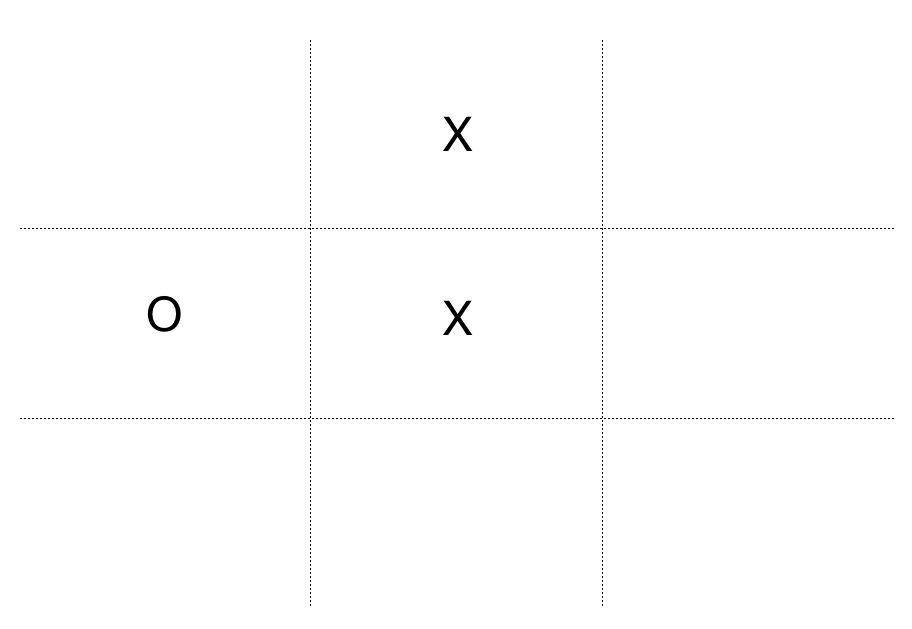
\includegraphics [scale=0.2] {ttt_5.png}
	\caption{}
	\label{Rys28}
\end{figure} 
$\text{Obserwacja po drugim ruchu agenta:  }[0, 2, 0, 1, 2, 0, 0, 0, 0, 0.723, 0]$\\

System - gracz losowy - w kolejnym ruchu nie blokuje agenta, tylko stawia kółko na pozycji $3,3$. W odpowiedzi na to, agent wybiera $3,2$ i wygrywa grę, stąd nagroda jest teraz równa $0.8$.

\begin{figure}[h!]
	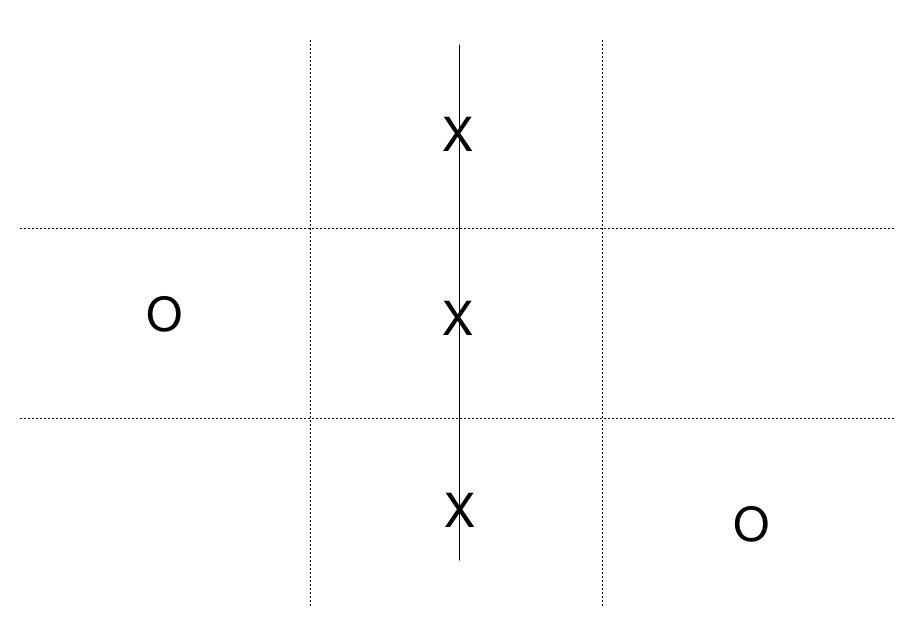
\includegraphics [scale=0.2] {ttt_8.png}
	\caption{}
	\label{Rys29}
\end{figure} 
$\text{Obserwacja po trzecim i ostatnim ruchu agenta ruchu agenta:  }[0, 2, 0, 1, 2, 0, 0, 2, 1, 0.843, 0.8]$\\

Powyższa gra dała w wyniku trzy obserwacje. Podczas jednej \textit{epoki} rozgrywamy tyle gier, żeby otrzymać 2500 obserwacji (albo tyle na ile ustalimy \textit{batch size}). Kolejnym krokiem jest zbudowanie na bazie tych obserwacji zbioru referencyjnego, na podstawie którego będziemy uczyć sieć. W tym celu zastąpimy prognozy $q_{s}$ jakie zwracała sieć ,,lepszymi'' wartościami $\tilde{q}_{s}$ wedle następującej reguły.  Ustalamy parametr $\alpha\in(0,1)$ i postępujemy jak następuje:


\begin{enumerate}
	\item{Jeżeli dana obserwacja jest ostatnią obserwacją w grze, to $\tilde{q}_{s}= R$}
	\item{W przeciwnym przypadku mamy  $N$ obserwacji pozyskanych w ramach aktualnie rozpatrywanej gry, gdzie $N$ jest ostatnią obserwacją.  Dla $i=N-1, N-2,...,1$ kładziemy: }
	\begin{enumerate}
		\item{$\tilde{q}_{N-i}= (1-\alpha^{i})q_{N-i} + \alpha^{i}q_{N} $}
	\end{enumerate}
\end{enumerate}
W skrajnym przypadku, jeżeli $\alpha=0$, to zmiana $\tilde{q}_{s}=q_{s}$ dla wszytskich stanów $s$, czyli nic się nie zmienia. W drugim skrajnym przypadku, jeżeli $\alpha=1$, to wszystkie $q_{s}$ z danej gry przyjmują wartość końcowej nagrody. Pomiędzy tymi skrajnościami modyfikujemy $q_{s}$ w zależności od końcowego wyniku gry, przy czym stany z początku gry są w mniejszym stopniu modyfikowane, aniżeli te bezpośrednio poprzedzające koniec gry.  \\

Stosując powyższą regułę do ciągu 2500 obserwacji otrzymujemy zbiór referencyjny, który po służy do uczenia sieci. Po przetrenowaniu sieci i aktualizacji wag, całą procedurę powtarzamy przez z góry ustaloną ilość epok. Poniżej przedstawiam wyniki jakie udało się uzyskać po 8 epokach, czyli bazując na 20 000 obserwacji.\\

\begin{figure}[h!]
	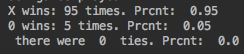
\includegraphics [scale=0.7] {nn2_1.png}
	\caption{Wynik trenowania sieci na 20 000 obserwacji w 8 epokach}
	\label{Rys30}
\end{figure} 

Jak widać agentowi na 100 gier udało się wygrać z graczem losowym w 95\% przypadków.  Można uznać, że to jest całkiem niezły wyniki, aczkolwiek w tym wypadku pomogła trochę losowość. Wydaje się, że średni procent wygranych gier plasuje się w okolicach 90\% przypadków. Poniżej (rysunek \ref{Rys31}) przykładowy wynik po 1000 grach. \\

\begin{figure}[h!]
	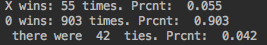
\includegraphics [scale=0.7] {nn2_2.png}
	\caption{}
	\label{Rys31}
\end{figure} 

A więc teraz agent gra dużo lepiej niż gracz losowy i ma lepsze wyniki niż sieć z I podejścia. Patrząc na wyniki gracza stosującego algorytm z 2 rozdziału (wygrane na poziomie 75\% -85\%)   można by przypuszczać, że sieć sobie radzi co najmniej nie gorzej. Nie jest to jednak poprawny wniosek. Algorytm z 2 rozdziału wygrywa rzadziej, ale też znacznie rzadziej przegrywa (w około 2\%) w stosunku do średnio 5\% przegranych w przypadku gracza bazującego na przetrenowanej sieci. Okazuje się, że ta różnica w ilości przegranych gier ma kluczowe znaczenie. Gracz ,,neuronowy'' prawie zawsze  przegrywa z graczem stosującym algorytm Q-learning z drugiego rozdziału. Na rysunku \ref{Rys32} zaprezentowano wyniki dla 100 rozegranych partii pomiędzy dwoma algorytmami:

\begin{figure}[h!]
	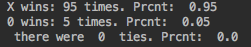
\includegraphics [scale=0.7] {nn2_3.png}
	\caption{Wynik 100 gier rozegranych pomiędzy graczem stosusującym Q-learning (X) i sieć neuronową (O)}
	\label{Rys32}
\end{figure} 

Warto jeszcze podkreślić, że algorytm z drugiego rozdziału stał się najbardziej efektywny po dodatkowych ,,sparingach'' z graczem  stosującym minimax. W wypadku sieci neuronowej dodatkowe trenowanie na bazie obserwacji uzyskanych podczas gier z graczem stosującym minimax nie przyniosło żadnej poprawy. Algorytm z rozdziału drugiego, przetrenowany dodatkowo na algorytmie minimax, prawie zawsze remisuje z graczem stosującym algorytm minimax, natomiast gracz wykorzystujący sieć neruonową już tylko w okolicach 40\%-50\% przypadków, co ilustruje (rysunek \ref{Rys32}) poniższy wynik rozegranych 100 gier.

\begin{figure}[h!]
	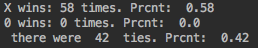
\includegraphics [scale=0.7] {nn2_4.png}
	\caption{Wynik 100 gier rozegranych pomiędzy graczem minimax (X) a graczem stosującym sieć neuronową (O)}
	\label{Rys33}
\end{figure} 

Reasumując, sieć nauczyła się skutecznie wygrywać z graczem losowym, ale niekoniecznie dobrze grać w kółko i krzyżyk, stąd pozostaje nieco słodko-gorzki smak po wykorzystaniu sieci neuronowych do gry w kółko i krzyżyk.\\

Na koniec podjęo jeszcze jedną próbę wytrenowania sieci bazując na zasadzie modyfikacji $q_{s}$ jak w I podejściu, ale tym razem nie trenując sieci w locie, po każdym ruchu, ale znowu rozgrywając tyle gier ile potrzeba do uzyskania 2500 obserwacji i trenowanie sieci dopiero na pełnym zbiorze obserwacji. Dokładniej,  $q_{s}$ czyli oczekiwaną wartość przyszłych nagród dla planszy w stanie $s$ po ruchu agenta z $s-1$ do $s$, modyfikowano zgodnie z regułą (zobacz \cite{RL} rozdział 6.5):

$$q_{s} := q_{s} + \alpha(R_{s}+\gamma\max_{s+1}q_{s+1}-q_{s}),$$

gdzie podobnie jak w poprzednich rozdziałach $\alpha$ to parametr sterujący szybkością uczenia się algorytmu (\textit{learning rate}), $\gamma$ to parametr dyskontujący przyszłe nagrody, $R_{s}$ to nagroda po odpowiedzi systemu na ruch agenta z $s-1$ do $s$. Niestety, tak jak w poprzednim podejściu, trenując sieci na 20 000 obserwacji (8 epizodów) udało się uzyskać wyniki rzędu 70\%  wygranych, 20\% przegranych i 10\% remisów z graczem losowym. A więc wyniki porównywalne z tymi uzyskanymi w podejściu I. Nieznaczna poprawa może wynikać z dodatkowej warstwy ukrytej. 
  

\chapter{Podsumowanie}
Celem pracy było zaimplementowanie i opisanie kilku wybranych algorytmów grających w grę ,,kółko i krzyżyk" i ten cel został osiągnięty,  aczkolwiek w przypadku algorytmu bazującego na sieciach neuronowych, poziom gry pozostawia wiele do życzenia.  W poniższych akapitach opisano po krótce, każdy z trzech algorytmów wraz z refleksjami odnośnie ich skuteczności,  możliwych ulepszeń w samym algorytmie lub w sposobie implementacji.\\

Minimax jest najbardziej klasycznym podejściem w przypadku gier z dwoma graczami o zerowej sumie nagród,  czyli gier, w których maksymalizacja wygranej jednego z graczy jest równoważna z minimalizacją wygranej oponenta.   Mimo, że kółko i krzyżyk składa się maksymalnie z 9 sekwencji ruchów, a więc drzewo gry ma 9 poziomów, to algorytm wydaje się ciężki i gra zajmuje dosyć długo . Grając z komputerem trudno to odczuć, ale ewidentnie do widać podczas trenowania innych algorytmów poprzez grę z graczem grającym minimax. Np. rozegranie na domowym komputerze autora 1000 gier pomiędzy dwoma graczami grającymi losowo zajmuje kilka sekund, a rozegranie 1000 gier pomiędzy graczem grającym losowo z graczem grającym minimax, to już są minuty. Gdyby dodać jeszcze jeden poziom do gry (takie kółko i krzyżyk na planszy 4 razy 4), to oczekiwanie na ruch komputera byłoby nie do zaakceptowania. W takim przypadku trzeba by koniecznie kończyć przeszukiwanie drzewa na jakimś wcześniejszym poziomie, tak jak to robią algorytmy grające w szachy.  Nieznaczną poprawę szybkości działania przyniosło w przycinanie $\alpha-\beta$. W pojedynczej grzez z komputerem nie daje się tego odczuć, ale przy ,,masowym" rozgrywaniu 1000 jest to nieznacznie szybciej. Podobno najlepsze algorytmy grające w szachy przeszukują drzew gry do 12-13 poziomów, więc pewnie poprawiając struktury danych na bardziej optymalne dało by się odciążyć i przyspieszyć tą implementację.\\

Największym pozytywnym zaskoczeniem był algorytm  \textit{Q- table} bazujący na algorytmie \textit{Off-policy Temporal Difference(0)} opisanym w rozdizale 6.5 w \cite{RL}. Zaczynając z pustą tabelą wartości $q_{s}$ już po 5000 gier mamy tabela wypełnia się około 600-700 stanami z odpowiadającymi im $q_{s}$ i algorytm wygrywa z graczem losowym w ponad 70\% przypadków. Trenowanie algorytmu na 20 000 grach skutkuje graczem na zbliżonym do człowieka. W zakresie implementacji kluczową rzeczą było, żeby nie otwierać i nie zamykać pliku z  tabelą  ze stanami i wartościami $q_{s}$ ponieważ jest to czasochłonne i opóźnia działanie programu. Czy to przy  jednorazowej grze (człowieka z graczem posługującym się algorytmem Q-table), czy przy trenowaniu algorytmu podczas wielu grach,  plik jest otwierany na początku, następnie przez całą sesję przetrzymywany w pamięci jest słwonik Q-table, i na końcu jest zapisywany do pliku.\\ 

Po sukcesach z algorytmem Q-table, wydawało się, że łatwo uda się wytrenować prostą sieć neuronową, która zamiast posługiwać się danymi tabelarycznymi (zapisywanymi do pliku), skompresuje tą informację w macierzach z wagami sieci. Niestety rzeczywistość nie potwierdziła tych optymistycznych założeń i trenując sieć na różne sposoby nie sposób było oprzeć się wrażenie dosięgania,,szklanego sufitu", którego nie udało się przebić. Istotnym jest pytania, co jeszcze można by potencjalnie zrobić, że nauczyć sieć dobrze grać w kółko i krzyżyk.  Na myśl przychodzi więcej warstw ukrytych oraz bardziej zaawansowane metody  sieciowo-neuronowe  typu    . Wydaje się jednak, że to idzie w kierunku strzelania z armaty do muchy. Sieć z jedną warstwą ukrytą jest w stanie całkiem dobrze rozpoznawać odręcznie pisane cyfry \cite{nn}. Trudno przypuszczać, żeby bądź co bądź banalna, gra w kółko i krzyżyk wymagałaby bardziej zaawansowanych metod. Może to kwestia dobrania odpowiednich hiper parametrów? Chociaż nie podjęto formalnych  prób przeszukiwania przestrzeni hiper parametrów, to raczej wątpliwym wydaje się być, żeby ich dobór mógł zaowocować prawdziwym przełomem.  W internecie można znaleść kilka ciekawych podejść, jednak większość  nie jest satysfakcjonujących. Jednym z takich podejść jest klasyfikowanie ruchów (dobry lub zły) za pomocą algorytmu minimax. Jeżeli gracz grający algorytmem minimax wybrałby ten ruch, to jest to dobry ruch, a w przeciwnym razie uznajemy ruch za zły. Następnie generując $n$ ruchów podczas gry z graczem losowym, możemy łatwo zbudować zbiór do trenowania sieci. Inne osoby z powodzeniem trenowały sieć korzystając z wcześniej ,,wytrenowanej" tabeli Q-table.  Takie drogi zupełnie mnie nie interesowała, jako że ogólnie wiadomo, że sieć można dobrze wytrenować (dopasaować o danych). Znacznie bardziej ciekawym pytaniem jest jak wykorzystać sieć neuronową do nauczenia się  jak grać w kółko i krzyżyk bez wspierania się już istniejącymi algorytmami; bez żadnej a priori wiedzy, poza samymi regułami gry. Stąd mój nacisk na trenowanie tylko i wyłącznie z graczem losowym, co w rezultacie dało całkiem niezłe wyniki przeciwko takiem graczu (ponad 90\%).  Jednak nie przełożyło się na umiejętność grania w potocznym, ludzkim, sensie. \\

Pierwotnie zamierzałem zająć się jeszcze jednym podejściem, a mianowicie algorytmem genetycznym. Zasadę działania takiego algorytmu można łatwo zobrazować. Na początku potrzebny jest relatywnie duży zbiór strategii $\pi_{i}$ indeksowany jakimś parametrem $i$. Następnie, losujemy pary strategii, której grają między sobą w kółko i krzyżyk. Pokonana strategia znika (ginie), a zwycięska może się reprodukować, ale potomstwo $\pi_{\tilde{i}}$ mutuje z pewnym prawdopodobieństwem. W efekcie otrzymujemy nowy zbiór strategii zawierający zwycięską strategię $\pi_{i}$ oraz jej potomstwo $\pi_{\tilde{i}}$.  Sekwencje rywalizacji a następnie reprodukcji z możliwością mutacji powtarzamy wielokrotnie, najlepiej aż do pozostania jednej, ewolucyjnie najlepszej strategii. Jak widać opis wydaje się prosty i zachęcający. Niestety trudności związane z wymyśleniem jak w ogóle charakteryzować strategie gry w kółko i krzyżyk, albo jak zapisać kod DNA danej strategii za pomocą parametrów będących obiektami matematycznymi, przerósł możliwości autora. 

\appendix

\chapter{Dodatek - opis kodu}
W tej części opisano podstawowe informacje dotyczące kodów napisanych w ramach niniejszej pracy oraz modułów (bibliotek) innych autorów , z których korzystano.  Nie  ma natomiast oposu poszczególnych elementów kodu i ich działania. Sam kod źródłowy, napisany w języku Python w wersji 2.17, stanowi załącznik do niniejszej pracy i można zorientować się za co odpowiadają poszczególne fragmenty czytając komentarze. Całość kodu składa się z kilku plików:
\begin{itemize}
	\item{\textbf{ttt.py} - zawiera implementację głównego programu i klas graczy}
	\item{\textbf{graphics.py} - moduł obsługujący grafikę autorstwa Johna Zelle \cite{Graphics}}
	\item{\textbf{neural.py} - moduł z implementacją sieci neuronowej w narzędziu \textit{Tensorflow}}
	\item{\textbf{QTable.txt} - plik tekstowy z wyuczonymi danymi dla algorytmu Q-Table}
	\item{ \textbf{ttt\_model.index, ttt\_model.meta, ttt\_model.data-000000-of-000001} - dane z wagami sieci neruonowej}
\end{itemize}

\section{Główny program}
Jądrem programu jest funkcja \textit{main()}, która jest odpowiedzialna za przeprowadzenie pojedynczej gry w kółko i krzyżyk. Funkcja przygotowuje planszę i zaznacza graficznie ruchy poszczególnych graczy, chyba że podając odpowiedni parametr wyłączy się grafikę, co jest niezbędne w przypadku rozgrywania tysięcy gier przy uczeniu algorytmów. Funkcja decyduje na podstawie podanych parametrów (domyślnie losowo) o tym, do którego gracza należy pierwszy ruch i wymaga wskazania dwóch graczy, przy czym mogą to być gracze stosujący różne algorytmy lub ludzie (w przypadku wybrania opcji włączonej grafiki). Funkcja \textit{main()} korzysta też z kilku funkcji pomocniczych, które sprawdzają, na przykład, czy po danym ruchu jest remis, czy gra się zakończyła wygraną  lub obsługują aktualizację grafiki. Program korzysta z elementarnych modułów \textit{random, sys, copy} oraz ze znanego modułu \textit{numpy} ułatwiającego obliczenia numeryczne, zwłaszcza w przypadku wielowymiarowych struktur danych, takich ja (n-wymiarowe) macierze.  

\section{Klasy graczy}
Opisana wyżej funkcja \textit{main()} wymaga przekazania jako argumentów dwóch instancji obiektów typu \textit{Player}, czyli obiektów reprezentujących graczy. Ogólnie, klasa typu \textit{Player} ma tylko jeden atrybut - symbol, który wskazuje czy gracz będzie grał kółkiem czy krzyżykiem. Natomiast każda ,,właściwy" typ gracza jest definiowany w osobnej podklasie:
\begin{enumerate}
	\item{Człowiek: klasa \textit{playerHuman}}
	\item{Gracz grający losowo: klasa \textit{playerRandom}}	
	\item{Cracz grający algorytmem minimax: klasa \textit{playerMinimax}}
	\item{Gracz grający algorytmem Q-Table: klasa \textit{playerQTable}}
	\item{Gracz grający z użyciem sieci neuronowej: klasa \textit{playerNeural}}
\end{enumerate}
Każda z tych podklas klasy \textit{Player} ma jedną główną metodę \textit{move()}, która przyjmuje stan  gry jako argument i wybiera najlepszy według siebie ruch. W przypadku klasy \textit{playerHuman} metoda \textit{move()} śledzi pozycję kursora i sprawdza gdzie na  planszy nastąpiło kliknięcie.  \\

Gdyby była potrzeba dodania kolejnej wersji algorytmu grającego w kółko i krzyżyk, np. algorytmu genetycznego, to poza dodaniem odpowiedniej opcji w GUI gry, ,,wystarczyłoby" dodać nową podklasę \textit{playerGenetic} ze stosowną metodą \textit{move()}, która przyjmuje głównie 9 elementowy ciąg 0,1 i 2 obrazujący sytujację na planszy i zwraca cyfrę od 1 do 9, która oznacza wybrane pole do ruchu.  

\section{Grafika}
Istnieje wiele modułów pozwalających tworzenie obiektów graficznych w Pythonie. Jako, że gra w kółko i krzyżyk nie jest graficznie wymagająca, to skorzystałem z bodajże najprostszego narzędzia napisanego przez Johna Zelle \cite{Graphics}. Podobno ten moduł został stworzony nie tyle z myślą o poważnych zastosowaniach graficznych, ale z myślą żeby uczyć programowania obiektowego na bazie prostych graficzyncyh obiektów typu punkt, linia, koło itp.  Ogólnodostępny kod źródłowy tego modułu graficznego można znaleźć na stronie \cite{Graphics}.

\section{Tensorflow}
Pierwotnym zamysłem była implementacja  sieci neuronowej od początku do końca za pomocą podstawowych modułów python'a. I mimo pewnych sukcesów na tym polu, ostatecznie zwyciężył pragmatyzm i sieci neuronowe opisana w rozdziale 3 powstały z wykorzystaniem bibliotek \textit{Tensorflow}. Jest to narzędzie stworzone przez potentata Google, i służy ogólnie do budowania grafów, w których węzłach mają miejsce obliczenia (w tym różnego typu optymalizacje), natomiast krawędzie ilustrują przepływ danych pomiędzy obliczeniami. Praca z tym narzędzie polega na zbudowaniu lub wczytaniu grafu, następnie zapewnienie niezbędnych danych wejściowych, przeprowadzeniu obliczeń po kolei zgodnie ze strukturą grafu i odczytaniu wyniku.  Więcej o o module \textit{Tensorflow} oraz o dostępnym w python'ie API  \textit{Tensorflow}do  można się dowiedzieć na oficjalnej stronie \cite{TF}.


\chapter{Dodatek - opis aplikacji}

Niezależnie od statystycznych wyników, jakie poszczególne algorytmy osiągają grając w kółko i krzyżyk, ciekawie jest samemu przekonać sie o 
skuteczności algorytmu grając z nim ,,osobiście". Taka ciekawość była główną motywacją do przygotowania w ramach niniejszej pracy 
bardzo prostej aplikacji gry w kółko o krzyżyk, która zostałą opisana w tym dodatku. \\

Aplikacja ma tylko jeden ekran (zobacz rysunek \ref{Rys34}), przedstawiający planszę do gry w kółko i krzyżyk. Po uruchomieniu aplikacji 
należy za pomocą niebieskich przycisków umieszczonych na dole planszy wybrać przeciwnika. Do wyboru można grać z drugą osobą (człowiekiem), 
z graczem grającym w sposób losowy,  graczem stosującym algorytm minimax, stosującym algorytm Q-Table lub graczem wykorzystującym sieć neuronową 
z 3 rodziału. Dodatkowo w prawym dolnym rogu aplikacja informuje o tym, którego gracza jest obecnie ruch.

\begin{figure}[h!]
	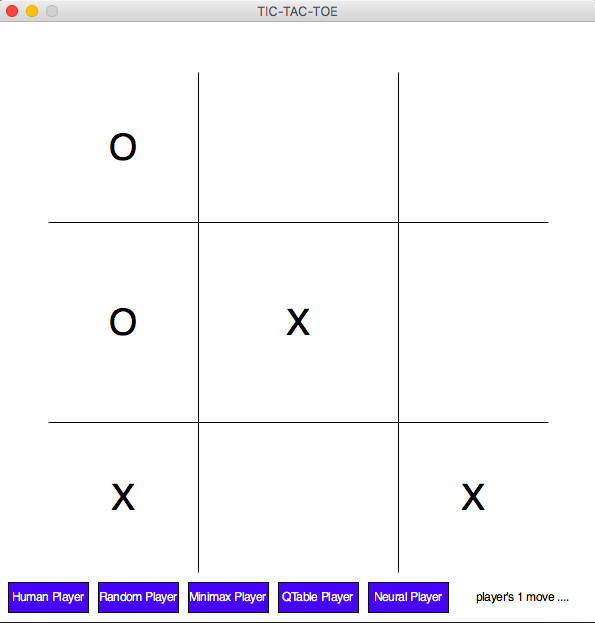
\includegraphics [scale=0.45] {plansza.png}
	\caption{Plansza do gry w kółko i krzyżyk}
	\label{Rys34}
\end{figure} 

W celu uruchomienia aplikacji trzeba mieć na komputerze zainstalowanego Pythona 2. Dodatkowo należy w jednym wybranym katalogu umieścić następujące 
pliki:
\begin{enumerate}
	\item{ttt.py}
	\item{graphics.py}
	\item{neural.py}
	\item{Qtable.txt}
	\item{ttt\_model.meta}
	\item{ttt\_model.index}
	\item{ttt\_model.data-00000-of-00001}
\end{enumerate}


Pliki 4 - 7 przechowują parametry wytrenowanych algorytmów Qtable i sieci neuronowej. Jeżeli tych plików zabraknie, to aplikacja będzie działała, ale gracze stosujący Q-Table lub sieć neruronową będą grali tak jak gracz losowy. Samo uruchomienie aplikacji odbywa się przez uruchomienie (otworzenie) pliku ttt.py za pomocą programu Python. Jeżeli dysponujemy rozbudowanym środowiskiem programistycznym (jak np. PyCharm) to można otworzyć otwprzyć plik korzystając ze stosownego okna dialogowego. W przeciwnym razie można posłużyć się wierszem poleceń tak jaj na rysunku \ref{Rys35}. 


\begin{figure}[h!]
	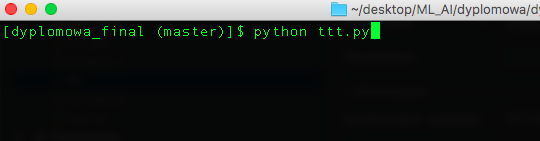
\includegraphics [scale=0.5] {uruchamianie.png}
	\caption{Uruchomienie aplikacji z wiersza poleceń}
	\label{Rys35}
\end{figure} 


Moduł ttt.py może również służyć do trenowania algorytmów QTable i sieci neuronowej, ale do tego nie ma GUI i konieczna jest zmiana wybranych parametrów w kodzie. 

\begin{thebibliography}{99}

\addcontentsline{toc}{chapter}{Bibliografia}

	\bibitem {nn} Michael Nielsen, \textit{Neural Networks and Deep Learning}, Determination Press, 2015
	
	\bibitem {itsl} James Gareth, \textit{Introduction to Statistical Learning}, Springer, 2013
	
	\bibitem {RL} Richard S. Sutton and Andrew G. Barto, \textit{Reinforcement Learning: An Introduction},  MIT Press, Cambridge, MA, 2018
	
	\bibitem {MIT_AI} Prof. Patrick Henry Winston, \textit{MIT course number 6.043, Artifical Inteligence}, https://ocw.mit.edu/courses/electrical-engineering-and-computer-science/6-034-artificial-intelligence-fall-2010/index.htm

	\bibitem{TUM} Michael Heining, \textit{Dynamic Learning: A case study on Tic-Tac-Toe}, https://www-m15.ma.tum.de/foswiki/pub/M15/Allgemeines/PublicationsEN/MasterThesisHeining.pdf
	
	\bibitem{Watkins} Christopher John Cornish Hellaby Watkins, \textit{Learning from Delayed Rewards}, http://www.cs.rhul.ac.uk/~chrisw/new\_thesis.pdf
	
	\bibitem{Game}  Matthew O. Jackson, \textit{A Brief Introduction to the Basics of Game Theory}, \linebreak https://ethz.ch/content/dam/ethz/special-interest/gess/chair-of-sociology-dam/documents/education/spieltheorie/literatur/Einf\%c3\%bchrung/\linebreak Jackson\%20Basics\%20of\%20Game\%20Theory\%20SSRN-id1968579.pdf

	\bibitem{Graphics} John Zelle,  \textit{Pyhton Programming: An introduction to Computer Science}, https://mcsp.wartburg.edu/zelle/python/
	\bibitem{TF} TensorFlow, https://www.tensorflow.org/
	

\end{thebibliography}

\end{document}


%%% Local Variables:
%%% mode: latex
%%% TeX-master: t
%%% coding: latin-2
%%% End:
